\chapter{Background}
\label{chap:background}

In this chapter we formally describe the concepts and the background information
needed to understand what follows.
In Section~\ref{sec:math-bg} we give some basic mathematical background;
in Section~\ref{sec:formal-langs} we introduce the concept of \emph{formal language}
and we characterize some classes of languages in which we are interested in;
in Section~\ref{sec:order-theory} we present basic notions of \emph{order theory};
in Section~\ref{sec:simulation} we define a number of \emph{simulation preorders}
on the states of an automaton and, finally,
in Section~\ref{sec:solving-inclusion} we describe how to solve the language
inclusion problem for certain classes of languages using
\emph{complete abstractions}.

\section{Mathematical background}
\label{sec:math-bg}

Let $X$ and $Y$ be two sets.
We denote by $|X|$ the \emph{cardinality} of $X$ and by $\powerset(X)$ its \emph{powerset}.
We define
$\fpowerset(X) \overset{\triangle}{=} \{S \in \powerset(X) \;|\; |S| < \infty\}$.
If $X$ is a subset of some universe set $U$ then $X^C$ denotes the complement of $X$
with respect to $U$ when $U$ is implicitly given by the context.
A \emph{partition} $P$ of $X$ is a set of non empty subsets of $X$, called \emph{blocks},
that are pairwise disjoint and whose union gives $X$.
If $f: X \rightarrow Y$ is a function between sets and $S \in \powerset(X)$ then
$f(S) \overset{\triangle}{=} \{f(x) \;|\; x \in S\}$ denotes its image on a
subset $S$.
A composition of two functions $f$ and $g$ is denoted both by $fg$ and $f \circ g$.
We define $id: X \rightarrow X$ as the \emph{identity function}, namely
$id(x) \eqdef x$.
Let $f: X \rightarrow X$ be a function.
For all $n \in \mathbb{N}$ we inductively define:
\[ f^n \eqdef
\begin{cases}
id & \textrm{if } n = 0\\
f \circ f^{n-1} & \textrm{if } n > 0
\end{cases}\]

One \emph{relation} $\mathscr{R}$ over $X$ is a subset of $X \times X$.
The \emph{composition} of two relations $\mathscr{R}_1,\mathscr{R}_2$ is
$\mathscr{R}_1 \circ \mathscr{R}_2 \; \eqdef \{(x,z) \;|\; \exists (x,y) \in \mathord{\mathscr{R}_1}\; \wedge \; \exists (y,z) \in \mathord{\mathscr{R}_2  }\}$.
Let $\mathscr{R}$ be a relation on $X$.
\begin{itemize}
\item $\mathscr{R}$ is \emph{reflexive} if for all $x \in X, x \mathscr{R} x$;
\item $\mathscr{R}$ is \emph{transitive} if for all $x,y,z \in X, x \mathscr{R} y \; \wedge \; y \mathscr{R} z \Longrightarrow x \mathscr{R} z$;
\item $\mathscr{R}$ is \emph{symmetric} if for all $x,y \in X, x \mathscr{R} y \Longleftrightarrow y \mathscr{R} x$;
\item $\mathscr{R}$ is \emph{antisymmetric} if for all $x,y \in X, x \mathscr{R} y \; \wedge \; y \mathscr{R} x \Longrightarrow x = y$.
\end{itemize}

If $\mathscr{R}$ is reflexive, transitive and symmetric we say that $\mathscr{R}$ is an \emph{equivalence}.
If $\mathscr{R}$ is reflexive, transitive and antisymmetric we say that
$\mathscr{R}$ is a \emph{partial order}.
If $\mathscr{R}$ is reflexive and transitive we say that $\mathscr{R}$ is a
\emph{quasiorder}, and we will recall this concept in Section~\ref{sec:order-theory}.
We define $[x]_{\mathscr{R}} \eqdef \{y \in X \;|\; x \mathscr{R} y \; \wedge \; y \mathscr{R} x\}$.
The \emph{transitive closure} of one relation $\mathscr{R}$ on one set $X$
is defined as the
smallest relation on $X$ that contains $\mathscr{R}$ and is transitive.
Let $\mathscr{R}_1,\mathscr{R}_2$ be two relations.
If $\mathord{\mathscr{R}_1} \subseteq \mathord{\mathscr{R}_2}$ we say that $\mathscr{R}_1$ is \emph{finer} than $\mathscr{R}_2$
and if $\mathord{\mathscr{R}_2} \subseteq \mathord{\mathscr{R}_1}$  we say that $\mathscr{R}_1$ is \emph{coarser} than $\mathscr{R}_2$.

Let $k \in \mathbb{N}$ and $x_1, \dots, x_k \in X$.
We denote by $\vec{x}$ the $k$-dimensional vector $\angles{x_i}_{i \in [1,k]} \in X^k$.
We denote by $(\vec{x})_i$ the element $x_i$.
In what follows we abuse notations by implicitly lifting them to vectors.
For instance, $\vec{x} \leq \vec{y} \iffdef \forall i \in [1,k], x_i \leq y_i$.
Sometimes we also implicitly lift the empty set $\emptyset$ to a vector,
writing $\emptyset$ to refer to
$\vec{\emptyset} \eqdef \angles{\emptyset}_{i \in [1,k]} \in \powerset(X)^k$.

\section{Formal languages}
\label{sec:formal-langs}

In mathematics, computer science, and linguistics, a \emph{formal language} consists
of words whose letters are taken from an alphabet $\Sigma$ and are
well-formed according to a specific set of rules.
The alphabet $\Sigma$ of a formal language consist of symbols that
concatenate into strings of the language.
Each string concatenated from symbols of this alphabet is called a \emph{word},
and the words that belong to a particular formal language are sometimes
called well-formed words or well-formed formulas.
A formal language is often defined by means of a formal grammar, such as a
regular grammar or context-free grammar, which consists of its formation rules.
We now describe these concepts more formally.

Let $\Sigma$ be a finite set of symbols.
A finite sequence of elements of $\Sigma$ is called a \emph{finite word}.
We denote the sequence $(a_1, a_2, \dots, a_n)$ by mere juxtaposition:
\[a_1a_2\dots a_n\]
The set of words is endowed with the operation of \emph{concatenation product},
which associates two words $u = a_1 a_2 \dots a_n$ and $v = b_1 b_2 \dots b_m$
the word $uv = a_1 a_2 \dots a_n b_1 b_2 \dots b_m$.
We denote with $\epsilon$ the \emph{empty word}.
We denote by $\Sigma^*$ the set of words on $\Sigma$ and by $\Sigma^+$ the set of
nonempty words, that is $\Sigma^+ \eqdef \Sigma^* \setminus \{\epsilon\}$.
An \emph{infinite word} on the alphabet $\Sigma$ is an infinite sequence of elements
of $\Sigma$, which we also denote by juxtaposition:
\[a_1 a_2 \dots a_n \dots \]
We denote with $\Sigma^{\omega}$ the set of infinite words over the alphabet
$\Sigma$.
One \emph{formal language}, or simply a \emph{language}, is a subset of
$\Sigma^*$ or $\Sigma^{\omega}$.
Let $L$ be a language, $w \in \Sigma^*$, we define
the \emph{context} of $w$ as
$ctx_{L}(w) \overset{\triangle}{=} \{(x,y) \in \Sigma^* \times \Sigma^* \; | \; xwy \in L\}$.


In the following sections we describe three classes of languages:
\emph{regular}, \emph{context-free} and
\emph{$\omega$-regular}.

\subsection{Regular languages and finite automata}

There are many different ways to defines regular languages.
A \emph{regular language} is a formal language that can be expressed using a
\emph{regular expression}~\cite{hopcroft2013introduction}.
The words of a regular language are sequences of finite length of symbols
in the alphabet $\Sigma$ .
An alternative definition of regular language is that a
regular language is the language accepted by \emph{finite automaton} (FA).
A FA can either be \emph{deterministic} or \emph{nondeterministic}.

A \emph{deterministic finite automaton} (DFA) is a tuple
$\automa{A}$ where $\Sigma$ is a finite alphabet, $Q$ is a finite set of states,
$I \; \subseteq Q$ is the set of \emph{initial} states, $F \; \subseteq Q$ is
the set of \emph{accepting}  states, and $\delta \; \subseteq Q \times \Sigma \times Q$
is the transition \emph{function}.
Figure~\ref{fig:DFA-example-1} shows an example of DFA.
A \emph{nondeterministic finite automaton} (NFA) is a tuple
$\automa{A}$ where $\Sigma$ is a finite alphabet, $Q$ is a finite set of states,
$I \; \subseteq Q$ is the set of \emph{initial} states, $F \; \subseteq Q$ is
the set of \emph{accepting}  states, and $\delta \; \subseteq Q \times \Sigma \times Q$
is the transition \emph{relation}.
Figure~\ref{fig:NFA-example-1} shows an example of NFA.
Observe that the difference between a DFA and a NFA is that in the former
$\delta$ is a function, while in the latter $\delta$ is a relation.

\begin{figure}[h]
\centering
\begin{tikzpicture}[shorten >=1pt,node distance=3cm,auto]
  \tikzstyle{every state}=[fill={rgb:black,1;white,10}]
  \node[state,initial] (q_0) {$q_0$};
  \node[state] (q_1) [above right of=q_0]  {$q_1$};
  \node[state,accepting] (q_2) [below right of=q_0]  {$q_2$};
  \path[->]
  (q_0) edge node {$a$} (q_1)
  (q_0) edge node {$b$} (q_2)
  (q_1) edge [loop above] node {$b$} (q_1)
  (q_1) edge node {$c$} (q_2)
  (q_2) edge [loop below] node {$b$} (q_2)
  ;
\end{tikzpicture}
\caption{Example of a DFA}
\label{fig:DFA-example-1}
\end{figure}

\begin{figure}[h]
\centering
\begin{tikzpicture}[shorten >=1pt,node distance=3cm,auto]
  \tikzstyle{every state}=[fill={rgb:black,1;white,10}]
  \node[state,initial] (q_0) {$q_0$};
  \node[state] (q_1) [above right of=q_0]  {$q_1$};
  \node[state,accepting] (q_2) [below right of=q_0]  {$q_2$};
  \path[->]
  (q_0) edge node {$a$} (q_1)
  (q_0) edge node {$a$} (q_2)
  (q_1) edge [loop above] node {$b$} (q_1)
  (q_1) edge node {$b$} (q_2)
  (q_2) edge [loop below] node {$b$} (q_2)
  ;
\end{tikzpicture}
\caption{Example of a NFA}
\label{fig:NFA-example-1}
\end{figure}

Let $q,q' \in Q$ and $a \in \Sigma$.
If $q' \in \delta(q,a)$ we write that $q \overset{a}{\rightarrow} q'$ and
if $\nexists q' \in \delta(q,a)$ we write that $q \overset{a}{\nrightarrow}$.
If $w \in \Sigma^*$, then
$q \goes{w} q'$ means that the state $q'$ is reachable from $q$ by following
the string $w$.
More formally, by induction on the length of $w$:
(i) if $w = \epsilon$ then $q \goes{\epsilon} q' \Longleftrightarrow q = q'$;
(ii) if $w = av$ with $a \in \Sigma$,  $v \in \Sigma^*$ then
$q \goes{av} q' \Longleftrightarrow \exists q'' \in \delta (q,a), q'' \goes{v} q' $.
We define $q \underset{u,q''}{\goes{uv}} q' \overset{\triangle}{\Longleftrightarrow} \exists q'' \in Q, q \goes{u} q'' \; \wedge \; q'' \goes{v} q'$.
When $q \goes{u} q' \; \wedge \; q' \goes{v} q''$ we write $q \goes{u} q' \goes{v} q''$.
We write $q \goesf{w} q'$ to denote the fact that the
state $q'$ is reachable from $q$ by following the string $w$, reaching at some
point one final state.
More formally, by induction on the length of the word $w$:
(i) if $w = \epsilon$, then $q \goesf{\epsilon} q'$ iff $q = q'$ and $q \in F$;
(ii) if $w = av$, then $q \goesf{av} q'$ iff $\exists q'' \in Q$ such that
$((q \in F \; \vee q'' \in F) \; \wedge \; q \trans{a} q'' \; \wedge \; q'' \goes{v} q')$
or $(q \trans{a} q'' \; \wedge \; q'' \goesf{v} q')$.
The \emph{language accepted by the FA $\mathcal{A}$} is
$\mathcal{L}(\mathcal{A}) \overset{\triangle}{=} \{w \in \Sigma^* \; | \; \exists q_i \in I, \exists q_f \in F, q_i
\goes{w} q_f\}$.
Figure~\ref{fig:DFA-example-2} shows an example of an automaton
accepting the language $a(b^*(ca)^*)^*$.

\begin{figure}[h]
\centering
\begin{tikzpicture}[shorten >=1pt,node distance=3cm,auto]
  \tikzstyle{every state}=[fill={rgb:black,1;white,10}]

  \node[state,initial] (q_0) {$q_0$};
  \node[state,accepting] (q_1) [right of=q_0]  {$q_1$};
  \path[->]
  (q_0) edge [bend left=45] node {$a$} (q_1)
  (q_1) edge [loop above] node {$b$} (q_1)
  (q_1) edge [bend left=45] node {$c$} (q_0)
  ;
\end{tikzpicture}
\caption{DFA accepting the language $a(b^*(ca)^*)^*$}
\label{fig:DFA-example-2}
\end{figure}

Let $S,T \subseteq Q$, we define $W_{S,T}^{\mathcal{A}} \overset{\triangle}{=} \{w \in \Sigma^* \; | \;
\exists p \in S, \exists q \in T, p \goes{w} q \}$.
When $S = \{p\}$ or $T = \{q\}$ we slightly abuse the notation writing $W_{p,T}^{\mathcal{A}}$,
$W_{S,q}^{\mathcal{A}}$ or $W_{p,q}^{\mathcal{A}}$.
Let $w \in \Sigma^*$ and $S \subseteq Q$, we define $ctx_{\mathcal{A}}(w) \overset{\triangle}{=}
\{(p,q) \in Q \times Q \; | \; p \goes{w} q \}$,
$ctx_{\mathcal{A}}^F(w) \overset{\triangle}{=} \{(p,q) \in Q \times Q \; | \; \exists p_f \in F,
w_1, w_2 \in \Sigma^*: p \goes{w_1} p_f \; \wedge \; p_f \goes{w_2}, w = w_1w_2 \}$,
$pre_w^{\mathcal{A}}(S) \overset{\triangle}{=} \{q \in Q \; | \; w \in W_{q, S}^{\mathcal{A}}\}$ and
$post_w^{\mathcal{A}}(S) \overset{\triangle}{=} \{q \in Q \; | \; w \in W_{S, q}^{\mathcal{A}}\}$.

$\mathcal{A}^{R} \overset{\triangle}{=} \langle Q, \Sigma, \delta^{R}, F, I \rangle$
is the \emph{reverse} of $\mathcal{A}$, where
$q \in \delta^{R}(q',a) \Longleftrightarrow q' \in \delta (q,a)$.
If $q' \in \delta^R(q,a)$ we write that $q \overset{a}{\rightarrow}_R q'$.
By induction on the length of $w$ we define what means $q \goes{w}_R q'$:
(i) if $w = \epsilon$ then $q \goes{\epsilon}_R q' \Longleftrightarrow q = q'$;
(ii) if $w = av$ with $a \in \Sigma$,  $v \in \Sigma^*$ then
$q \goes{av}_R q' \Longleftrightarrow \exists q'' \in \delta^R (q,a), q'' \goes{v}_R q' $.
Figure~\ref{fig:reverse-example} shows the reverse of the DFA in
Figure~\ref{fig:DFA-example-2}.

\begin{figure}[h]
\centering
\begin{tikzpicture}[shorten >=1pt,node distance=3cm,auto]
  \tikzstyle{every state}=[fill={rgb:black,1;white,10}]

  \node[state,accepting] (q_0) {$q_0$};
  \node[state,initial] (q_1) [right of=q_0]  {$q_1$};
  \path[->]
  (q_1) edge [bend right=45, above] node {$a$} (q_0)
  (q_1) edge [loop above] node {$b$} (q_1)
  (q_0) edge [bend right=45, below] node {$c$} (q_1)
  ;
\end{tikzpicture}
\caption{Reverse of the DFA in Figure~\ref{fig:DFA-example-2}}
\label{fig:reverse-example}
\end{figure}


\begin{lemma}
\label{lemma:goes-retro}
Let $w \in \Sigma^*$ and $p,q \in Q$, then:
\[ p \goes{w} q \Longleftrightarrow q \goes{w^R}_R p \]
\end{lemma}

\begin{proof}
It follows from an induction on $|w|$.
If $|w|=0$, then $w = \epsilon$ and by the definition of $\rightsquigarrow$, $p=q$.
If $|w| > 0$, then $w=av=ub$, $w^R=v^Ra=bu^R$ for $a,b \in \Sigma$, $v,u \in \Sigma^*$
such that $av = ub$.
If $p \goes{av} q$, then $\exists p' \in Q$ such that $p \overset{a}{\rightarrow} p'$
and $p' \goes{v} q$.
For inductive hypothesis $q \goes{v^R}_R p'$, and since $p \overset{a}{\rightarrow} p'$
implies $p' \overset{a}{\rightarrow}_R p$, $q \goes{v^R a}_R p$.
If $q \goes{bu^R}_R p$, then $\exists q' \in Q$
such that $q \overset{b}{\rightarrow}_R q'$
and $q' \goes{u^R}_R p$.
For inductive hypothesis $p \goes{u} q'$,
and since $q \overset{b}{\rightarrow}_R q'$
implies $q' \overset{b}{\rightarrow} q$, $p \goes{ub} q$.
\end{proof}

\subsection{Context-free languages and context-free grammars}

In order to define context-free languages we have to introduce the concept of
context-free grammar.
A \emph{context-free grammar} (CFG) is a tuple $\mathcal{G} =\angles{\mathcal{V}, \Sigma, P}$
where $\mathcal{V} = \{X_0, X_1, \dots, X_n\}$ is the finite set of \emph{variables}
including the start symbol $X_0$,
$\Sigma$ is the finite alphabet of \emph{terminals} and
$P$ is is the set of productions $X_i \rightarrow \beta$ where
$\beta \in (\mathcal{V} \cup \Sigma)^*$.
We assume, for simplicity and without loss of generality,
that CFGs are in \emph{Chomsky Normal Form} (CNF),
that is, every production $X_i \rightarrow \beta \in P$ is such that
$\beta \in (\mathcal{V} \times \mathcal{V}) \cup \Sigma \cup \{\epsilon\}$
and if $\beta = \epsilon$ then $i = 0$~\cite{chomsky1959certain}.
We also assume that for all $X_i \in \mathcal{V}$ there exists a production
$X_i \rightarrow \beta \in P$, otherwise $X_i$ can be safely removed from $\mathcal{V}$.
Given two words $w,w' \in (\mathcal{V} \cup \Sigma)^*$ we write $w \rightarrow w'$
iff there exists $u,v \in (\mathcal{V} \cup \Sigma)^*$ and $X \rightarrow \beta$
such that $w = uXv$ and $w' = u\beta v$.
We denote by $\rightsquigarrow$ the reflexive-transitive closure of $\rightarrow$.
The language accepted by a CFG $\mathcal{G}$ is
$\lang{G} \eqdef \{w \in \Sigma^* \;|\; X_0 \rightsquigarrow w\}$.
Figure~\ref{fig:example-cfg} shows an example of CFG generating the language
$\{a^nb^n \;|\; n \geq 0\}$, while Figure~\ref{fig:example-cfg-chomsky} shows
a CFG that accepts the same language but is in CNF.
The class of languages accepted by CFGs is called \emph{contex-free languages}.

\begin{figure}[h]
\centering
\begin{equation*}
\begin{split}
X_0 \rightarrow \; & aX_0b \\
X_0 \rightarrow \; & \epsilon \\
\end{split}
\end{equation*}
\caption{CFG that accepts the language $\{a^nb^n \;|\; n \geq 0\}$}
\label{fig:example-cfg}
\end{figure}

\begin{figure}[h]
\centering
\begin{equation*}
\begin{split}
X_0 \rightarrow \; & X_2X_1 \\
X_0 \rightarrow \; & \epsilon \\
X_1 \rightarrow \; & X_0X_3 \\
X_2 \rightarrow \; & a \\
X_3 \rightarrow \; & b \\
\end{split}
\end{equation*}
\caption{CFG in \emph{Chomsky Normal Form} that accepts the language $\{a^nb^n \;|\; n \geq 0\}$}
\label{fig:example-cfg-chomsky}
\end{figure}


\subsection{$\omega$-regular languages and B{\"u}chi automata}
In order to define $\omega$-regular languages we have to introduce the concept
of B{\"u}chi automaton (BA).
The definition of BA is analogous to the definition of FA, they differ just on how
to accept words.
BAs can be \emph{deterministic} or \emph{nondeterministic}.

A \emph{deterministic B{\"u}chi automaton} (DBA) is tuple
$\automa{B}$ where $\Sigma$ is a finite alphabet, $Q$ is a finite set of states,
$I \; \subseteq Q$ is the set of \emph{initial} states, $F \; \subseteq Q$ is
the set of \emph{accepting}  states, and $\delta \; \subseteq Q \times \Sigma \times Q$
is the transition \emph{function}.
A \emph{nondeterministic B{\"u}chi automaton} (NBA) is tuple
$\automa{B}$ where $\Sigma$ is a finite alphabet, $Q$ is a finite set of states,
$I \; \subseteq Q$ is the set of \emph{initial} states, $F \; \subseteq Q$ is
the set of \emph{accepting}  states, and $\delta \; \subseteq Q \times \Sigma \times Q$
is the transition \emph{relation}.

In order to define the language accepted by BAs we have to introduce the concept
of \emph{trace}.
One \emph{infinite trace} of the automaton $\automa{B}$ on an infinite
word $w= a_0 a_1 \dots \in \Sigma ^{\omega}$ starting in a state $q_0 \in Q$
is an infinite sequence of transitions $\pi = q_0 \trans{a_0} q_1 \trans{a_1} \cdots$.
Similarly, a \emph{finite trace} on a finite word $w = a_0 a_1 \dots a_n \in \Sigma^*$
starting in a state $q_0 \in Q$ is a finite sequence of transitions
$\pi = q_0 \trans{a_0} q_1 \trans{a_1} \cdots \trans{a_n} q_{n+1}$.
A trace is \emph{initial} if it starts in an initial state $q_0 \in I$, and a finite trace is \emph{final}
if it ends in an accepting state $q_f \in F$.
A trace is \emph{fair} if it is infinite and $q_i \in F$ for infinitely many i's.
Differently from FAs, B{\"u}chi automata recognize languages of \emph{infinite} words.
In particular, the \emph{language} of a BA $\mathcal{B}$ is
$\lang{B} \overset{\triangle}{=} \{ w \in \Sigma ^{\omega} \; | \;
\mathcal{B} \textrm{ has an initial and fair trace on $w$}\}$.
Figure~\ref{fig:BA-example} shows an example of a B{\"u}chi automaton that
accepts the language $a^{\omega}$.
An \emph{$\omega$-regular language} is a language recognized by a B{\"u}chi
automaton.

\begin{figure}[h]
\centering
\begin{tikzpicture}[shorten >=1pt,node distance=3cm,auto]
  \tikzstyle{every state}=[fill={rgb:black,1;white,10}]
  \node[state,initial,accepting] (q_0) {$q_0$};
  \path[->]
  (q_0) edge [loop above] node {$a$} (q_0)
  ;
\end{tikzpicture}
\caption{B{\"u}chi automaton that accepts the language $a^{\omega}$}
\label{fig:BA-example}
\end{figure}

When the distinction between BAs and FAs is important we specify it,
otherwise assume that $\mathcal{A}$ is an automaton such that $\automa{A}$.
As a convertion, we will refer to FAs and generic automata as $\mathcal{A}$
and to BAs as $\mathcal{B}$.



\subsection{The language inclusion problem}

Deciding whether a formal language contains another one is a fundamental problem
in computer science with diverse applications including automata-based
verification~\cite{kupferman2018automata},
reasoning for logical theories~\cite{esparza2017automata}
or type systems~\cite{hofmann2014abstract}.
Typically, inclusion problems are computationally intensive.

Let $L_1, L_2$ be two languages.
The \emph{language inclusion problem} consists in checking if $L_1 \subseteq L_2$
holds.
Whether $L_1 \subseteq L_2$ is computable or not, depends on the nature
of $L_1$ and $L_2$.

It is well-known that if they are both regular the problem is computable,
and many algorithms have been proposed to check the
inclusion~\cite{ganty2019language, de2006antichains, abdulla2010simulation}.
This problem is PSPACE-complete~\cite{abdulla2010simulation}.
If $L_1$ is context-free and $L_2$ is regular the problem is still decidable.
In Section~\ref{sec:checking-grammars} we present the framework put forward in~\cite{ganty2019language}
to check this inclusion.

We are particularly in interested in the language inclusion problem
between $\omega$-regular languages.
It is known to be a PSPACE-complete~\cite{kupferman1996verification} problem and becomes
EXPTIME-complete~\cite{meyer2017liveness} when the ``smaller''
language is $\omega$-context free.
In Section~\ref{sec:checking-omega-lang-inc} we describe the framework
for checking the language inclusion between $\omega$-regular languages
proposed in~\cite{ganty2020omegalang}.

\section{Order theory}
\label{sec:order-theory}

Let $D$ be a set.
$\langle D, \leq \rangle$ is a \emph{quasiordered set} (qoset) when $\leq$
is a \emph{quasiorder} (qo) relation on $D$, that is, reflexive and transitive.
We sometimes refer to quasiorders as \emph{preorders}.
A qoset $\langle D, \leq \rangle$ is a \emph{partially ordered set} (poset)
when $\leq$ is antisymmetric.
The \emph{powerset} of $D$ is one example of poset.
A qoset satisfies the \emph{ascending} (resp. \emph{descending}) \emph{chain condition}
(ACC, resp. DCC) if there is no countably infinite sequence of distinct elements
$\{x_i\}_{i \in \mathbb{N}}$ such that, for all $i \in \mathbb{N}, x_i \leq x_{i+1}$
(resp. $x_{i+1} \leq x_i$).
An \emph{antichain} in a qoset $\angles{D,\leq}$ is a subset $X \subseteq D$ such that
any two distinct element  in $X$ are incomparable.
We denote the set of antichains of a qoset $\angles{D, \leq}$ by
$AC_{\angles{D,\leq}} \eqdef \{X \subseteq D \;|\; X \textrm{ is an antichain}\}$.
A qoset is called ACC (DCC) when it satisfies the ACC (DCC).
A qoset $\langle D, \leq \rangle$ is a \emph{well-quasiordered set} (wqoset)
when $\leq$ is a \emph{well-quasiorder} (wqo) relation  on $D$, that is,
when for every countably infinite sequence of elements $\{x_i\}_{i \in \mathbb{N}}$
there exist $i,j \in \mathbb{N}$ such that $i < j$ and $x_i \leq x_j$.
For every qoset $\angles{D,\leq}$, let us define the following binary relation
$\sqsubseteq$ on the $\powerset (D)$: given $X,Y \in \powerset(D)$,
$X \sqsubseteq Y \iffdef \forall x \in X, \exists y \in Y, y \leq x$.
A \emph{minor} of a subset $X \subseteq D$, denoted by $\minor{X}$, is a subset
of $X$ satisfying: (i) $X \sqsubseteq \minor{X}$ and (ii) $\minor{X}$ is an \emph{antichain}.
Let us recall that every subset of a wqoset $\angles{D,\leq}$has at least one minor set,
all minor sets are finite and if $\angles{D,\leq}$ is additionally a poset then
there exists \emph{exactly one} minor set.

Let $\langle D, \leq \rangle$ be a qoset.
An \emph{(upper) closure operator} on $D$, is a function in $D \rightarrow D$
that is monotone (i.e. $x \leq y \Longrightarrow \rho (x) \leq \rho(y)$),
idempotent (i.e., $\rho = \rho \rho$) and increasing
(i.e., $x \leq \rho(x)$).
The qoset $D$ induces a closure operator $\rho_{\leq}$ defined by
$\rho_{\leq}(X) \overset{\triangle}{=} \{ y \in D \;|\; \exists x \in X, x \leq y\}$.
We call $\rho_{\leq}(X)$ the \emph{upward closure} of $X$ and if $x \in X$
we abuse the notation and write $\rho_{\leq}(x)$ for $\rho_{\leq}(\{x\})$.

Let $\angles{D,\leq}$ be a poset.
Given two elements $x$ and $y$ in $D$, we call \emph{upper bound} of $x$ and
$y$ any element $z \in D$ such that $x \leq z$ and $y \leq z$.
Likewise, a \emph{lower bound} $z$ of $x$ and $y$ satisfies $z \leq x$ and
$z \leq y$.
Moreover, $z$ is the \emph{least upper bound}, also called \emph{lub} or \emph{join},
if it is the smallest element grater than both $x$ and $y$.
Such a upper bound does not necessarily exist but, when it does,
it is unique.
It is written as $x \sqcup y$.
Likewise, the unique \emph{greatest lower bound} of $x$ and $y$, also called
\emph{glb} or \emph{meet}, if it exists, is the greatest element smaller than
$x$ and $y$, and it is denoted as $x \sqcap y$.
As $\sqcup$ and $\sqcap$ are associative operators, we will employ also the
notations $\sqcup \; A$ and $\sqcap \; A$
to compute lubs an glbs on arbitrary (possibly infinite) sets $A$ of elements.
We denote respectively as $\bot$ (called \emph{bottom}) and $\top$ (called \emph{top})
the \emph{least element} and the \emph{greatest element} in the poset, if they exist.

A \emph{chain} $C \subseteq D$ in a poset $\langle D, \leq \rangle$ is a subset
$C$ of $D$ such that is totally ordered:
$\forall x,y \in C: (x \leq y) \; \vee \; (y \leq x)$.
A \emph{complete partial order} (CPO) is a poset such that every chain has a lub.

A \emph{lattice} $\langle D, \leq, \sqcup, \sqcap \rangle$ is a poset such that
$\forall x,y, \in D: x \sqcup y$ and $x \sqcap y$ exist.
A \emph{join-semilattice} $\angles{D, \leq, \sqcup, \bot}$ is a poset that
has the lub of all its arbitrary nonempty finite subsets.
A \emph{complete lattice} $\langle D, \leq, \sqcup, \sqcap, \bot, \top \rangle$
is a poset that has the lub of all its arbitrary
(possibly empty) subsets.

\subsection{Fixpoints}

Let $\langle D, \leq \rangle$ be a poset, $f : D \rightarrow D$ a function
and $x \in D$.
\begin{itemize}
\item  $x$ is a \emph{fixpoint} of $f$ if $f(x) = x$.
We denote as $fp(f) \eqdef \{x \in D \;|\; f(x) = x\}$ the set of fixpoints of $f$;
\item $x$ is a \emph{prefixpoint} of $f$ is $x \leq f(x)$;
\item $x$ is a \emph{postfixpoint} of $f$ is $f(x) \leq x$;
\item $\plfp{_x} f \eqdef min \{ y \in fp(f) \;|\; x \leq y\}$, if it exists, is the
\emph{least fixpoint} of $f$ greater than $x$;
\item $\lfp f \eqdef \plfp{_\bot f}$, is it exists, is the \emph{least fixpoint} of $f$;
\item $\pgfp{_x} f \eqdef max \{ y \in fp(f) \;|\; y \leq x\}$, if it exists, is the
\emph{greatest fixpoint} of $f$ greater than $x$;
\item $\gfp f \eqdef \pgfp{_\top f}$, is it exists, is the \emph{greatest fixpoint} of $f$.
\end{itemize}

In order to guarantee the existence of fixpoints we need some extra hypotheses
on $f$ and $\langle D, \leq \rangle$.
A function $f: \angles{D_1, \leq_1} \rightarrow \angles{D_2, \leq_2}$ between two
posets is \emph{monotonic} if
$\forall x,y \in D_1: x \leq_1 y \Longrightarrow f(x) \leq_2 f(y)$.
Monotonicity is related to the existence of fixpoints, as the following
Theorem states~\cite{tarski1955lattice}.

\begin{theorem}[Tarski's Theorem]
If $f: D \rightarrow D$ is a monotonic operator is a complete lattice
$\angles{D, \leq, \sqcup, \sqcap, \bot, \top}$, then the set of fixpoints
$fp(p)$ is a non-empty complete lattice.
In particular, $\lfp f$ exists.
Furthermore, $\lfp f = \sqcap \{x \in D \;|\; f(x) \leq x\}$.
\end{theorem}

A function $f: \angles{D_1, \leq_1, \sqcup_1} \rightarrow \angles{D_2, \leq_2, \sqcup_2}$
between two CPOs is \emph{continuous} if for every chain $C \subseteq D_1$,
$\{f(c) \;|\; c \in C\}$ is also a chain and the limits coincide:
$f(\sqcup_1 \; C) = \sqcup_2 \{ f(c) \;|\; c \in C\}$.
Another useful fixpoint theorem, found, e.g., in~\cite{cousot1977abstract},
is inspired by Kleene\cite{kleene1952introduction}'s star construction:

\begin{theorem}[Kleene's Theorem]
If $f: D \rightarrow D$ is a continuous function in a CPO
$\angles{D, \leq, \sqcup, \top}$, then $\lfp f$ exists.
Moreover, $\lfp f = \sqcup \{f^i(\bot) \;|\; i \in \mathbb{N}\}$.
\end{theorem}

This theorem requires stronger hypotheses on the function $f$ than Taski's Theorem,
but it does not require a complete lattice, only a CPO.
More interestingly, the iteration scheme makes the theorem \emph{constructive}:
one can imagine the process of computing iterations one by one from $\bot$.
Due to Kleene's Theorem, the following procedure provides the possibly
infinite sequence of so-called \emph{Kleene iterates} of the function $f$
starting from the basis $x$.

\[ \textrm{ \texttt{Kleene($f$,$x$)}} \eqdef
\begin{cases}
y \leftarrow x;\\
\textrm{\textbf{while}} f(y) \neq y \textrm{ \textbf{do}}\\
\;\;\;\;\;\;\;y \leftarrow f(y);\\
\textrm{\textbf{return }} y \\
\end{cases}\]

When $D$ is an ACC CPO and $f$ is monotonic, \texttt{Kleene($f$,$x$)} terminates
and returns the least fixpoint of the function $f$ which is greater than or
equal to $x$.
Moreover, under the same hypotheses \texttt{Kleene($f$,$\bot$)} returns the
lfp of the function $f$.

\subsection{Quasiorders on words}
\label{sec:qos-on-words}

A quasiorder $\leq$ on $\Sigma^*$ is \emph{left-monotonic} (\emph{right-monotonic})
if $\forall y, x_1,x_2 \in \Sigma^*, x_1 \leq x_2 \Longrightarrow yx_1 \leq yx_2$
($x_1y \leq x_2y$).
Also, $\leq$ is called \emph{monotonic} if it is both left and right-monotonic.

\begin{definition}[L-consistency]
Let $L \in \powerset(\Sigma^*)$ and $\leq_L$ be a quasiorder on $\Sigma^*$.
Then, $\leq_L$ is called left (resp. right) $ L-$consistent if and only if:
(i) $\leq_L \cap \; (L \times \neg L) = \varnothing$;
(ii) $\leq_L$ is left (resp.right) monotonic.
Furthermore, $\leq_L$ is called $L-$consistent when it is both left and right $L-$consistent.
\end{definition}

We see in Section~\ref{sec:checking-grammars} that if one qo monotonic and $L$-consistent,
then it can be used in the framework described in~\cite{ganty2019language}
to solve the language inclusion problem $L_1 \subseteq L_2$ where $L_1$ is
context-free and $L_2$ is regular.

We present some wqos defined in \cite{ganty2019language}.
Observe that $\dir$ is the direct simulation relation on states, while
$\revdir$ is the reverse simulation on states (see Section~\ref{sec:simulation}).
Let $L \in \powerset (\Sigma^*)$, $\mathcal{A}$ be an automaton, $u,v \in \Sigma^*$:
\[ u \leqq_{L} v \overset{\triangle}{  \Longleftrightarrow } ctx_L(u) \subseteq ctx_L(v)\]
\[ u \wss{A} v \overset{\triangle}{  \Longleftrightarrow } ctx_{\mathcal{A}}(u) \subseteq ctx_{\mathcal{A}}(v)\]
\[ u \wrdir{A} v \overset{\triangle}{\Longleftrightarrow}
    \forall q \in post_u^{\mathcal{A}}(I) \; \exists p \in post_v^{\mathcal{A}}(I) \textrm{ such that } q \dir p \]
\[ u \wldir{A} v \overset{\triangle}{\Longleftrightarrow}
    \forall q \in pre_u^{\mathcal{A}}(F) \; \exists p \in pre_v^{\mathcal{A}}(F) \textrm{ such that } q \revdir p \]
The first is known as the \emph{Myhill quasiorder}, while the second is
a \emph{state-based quasiorder}.
If $\mathcal{A}$ is a FA, they are both decidable monotonic wqos~\cite{ganty2019language} and
$\leqq_{A}$ is $L-$consistent.
Furthermore, also $\wss{A}$ is $\lang{A}$-consistent.
$\wrdir{A}$ is right-monotonic and $\wldir{A}$ is left-monotonic.
If $\mathcal{A}$ is a FA they are respectively right $\lang{A}$-consistent
and left $\lang{A}$-consistent.
They are both decidable wqos as well.

Some of these qos will be referenced frequently, in particular $\wss{A}$ will be used
in the framework for solving the language inclusion problem for $\omega$-regular
languages described in Section~\ref{sec:checking-omega-lang-inc}.
Furthermore, $\wrdir{A}$ is the first right-monotonic simulation-based qo
that we present.
In Chapter~\ref{chap:qos} we will generalize $\wrdir{A}$ in order
to obtain a number of different right-monotonic simulation-based qos.

\section{Simulation quasiorders on states}
\label{sec:simulation}

We assume that the automata are
\emph{forward} and \emph{backward} complete (or simply \emph{complete}),
i.e., for any state $p \in Q$
and symbol $a \in \Sigma$, there exist states $q_0,q_1 \in Q$ such that
$q_0 \trans{a} p \trans{a} q_1$.
In our examples not every automaton is backward and forward complete,
because otherwise they would be too complicated.
Observe that in the examples we can consider incomplete automata without loss
of generality:
as Proposition~\ref{proposition:complete-FA} and \ref{proposition:complete-BA} state,
every automaton can be converted into an equivalent complete one.

\begin{proposition}
\label{proposition:complete-FA}
Let $\mathcal{A} = \langle Q, \Sigma, \delta, I, F\rangle$ be a FA.
There exists a backward and forward complete FA $\mathcal{A}'$ such that
$\lang{A} = \mathcal{L}(\mathcal{A}')$.
\end{proposition}

\begin{proof}
We define $\mathcal{A}'$ in terms of the components $Q, \delta, I, F$ of $\mathcal{A}$:
\begin{itemize}
\item $Q' = Q \cup \{b, f\}$, where $b$ and $f$ are two new states;
\item $\delta' = \delta \cup \{(b,a,q) \;|\; \nexists (q', a, q) \in \delta\} \cup
\{(b, a, b) \;|\; a \in \Sigma \}\cup \{(q,a,f) \;|\; \nexists (q,a,q') \in \delta\}
\cup \{(f,a,f) \;|\; a \in \Sigma\}$;
\item $I' = I$;
\item $F' = F$.
\end{itemize}
The runs of $\mathcal{A}'$ are a superset of those of $\mathcal{A}$ since we
have added states and transitions.
Furthermore, on any input word $w$ the accepting runs of $\mathcal{A}$
and $\mathcal{A}'$ correspond, because any run that reaches $f$ stays in $f$,
and since $f \notin F'$, such a run can't reach a final state.
\end{proof}

\begin{proposition}
\label{proposition:complete-BA}
Let $\mathcal{B} = \langle Q, \Sigma, \delta, I, F\rangle$ be a BA.
There exists a backward and forward complete BA $\mathcal{B}'$ such that
$\lang{B} = \mathcal{L}(\mathcal{B}')$.
\end{proposition}

\begin{proof}
We define $\mathcal{B}'$ in terms of the components $Q, \delta, I, F$ of $\mathcal{B}$:
\begin{itemize}
\item $Q' = Q \cup \{b, f\}$, where $b$ and $f$ are two new states;
\item $\delta' = \delta \cup \{(b,a,q) \;|\; \nexists (q', a, q) \in \delta\} \cup
\{(b, a, b) \;|\; a \in \Sigma \}\cup \{(q,a,f) \;|\; \nexists (q,a,q') \in \delta\}
\cup \{(f,a,f) \;|\; a \in \Sigma\}$;
\item $I' = I$;
\item $F' = F$.
\end{itemize}
The runs of $\mathcal{B}'$ are a superset of those of $\mathcal{B}$ since we
have added states and transitions.
Furthermore, on any infinite input word $w$ the accepting runs of $\mathcal{B}$
and $\mathcal{B}'$ correspond, because any run that reaches $f$ stays in $f$,
and since $f \notin F'$, such a run is not fair.
\end{proof}

In the following example we show how to transform one incomplete FA
in a complete one.

\begin{figure}[h]
\centering
\begin{tikzpicture}[shorten >=1pt,node distance=3cm,auto]
  \tikzstyle{every state}=[fill={rgb:black,1;white,10}]

  \node[state,initial] (q_0) {$q_0$};
  \node[state] (q_1) [right of=q_0]  {$q_1$};
  \node[state,accepting] (q_2) [right of=q_1]  {$q_2$};

  \path[->]
  (q_0) edge node {$a$} (q_1)
  (q_1) edge [bend left, above left] node{$b$} (q_2)
  (q_2) edge [bend left] node  {$c$} (q_1)
  ;
\end{tikzpicture}
\caption{Incomplete FA accepting the language $ab(cb)^*$}
\label{fig:incomplete}
\end{figure}

\begin{figure}[h]
\centering
\begin{tikzpicture}[shorten >=1pt,node distance=3cm,auto]
  \tikzstyle{every state}=[fill={rgb:black,1;white,10}]

  \node[state,initial] (q_0) {$q_0$};
  \node[state] (q_1) [right of=q_0]  {$q_1$};
  \node[state,accepting] (q_2) [right of=q_1]  {$q_2$};
  \node[state] (b) [below of=q_1]  {$b$};
  \node[state] (f) [above of=q_1]  {$f$};

  \path[->]
  (q_0) edge node {$a$} (q_1)
  (q_1) edge [bend left, above left] node{$b$} (q_2)
  (q_2) edge [bend left] node  {$c$} (q_1)
  (b) edge node  {$a,b,c$} (q_0)
  (b) edge node {$b$} (q_1)
  (b) edge node {$a,c$} (q_2)
  (b) edge [loop below] node {$a,b,c$} (b)
  (q_0) edge node  {$b,c$} (f)
  (q_1) edge node  {$a,c$} (f)
  (q_2) edge node  {$a,b$} (f)
  (f) edge [loop above] node {$a,b,c$} (f)
  ;
\end{tikzpicture}
\caption{Complete FA accepting the language $ab(cb)^*$}
\label{fig:complete}
\end{figure}

\begin{example}
Let $\mathcal{A}$ be the FA in Figure~\ref{fig:incomplete}.
If we add states $b$ and $f$ and the transitions described in
Proposition~\ref{proposition:complete-FA} we obtain the FA
$\mathcal{A}'$ in Figure~\ref{fig:complete}.
It is easy to check that $\lang{A} = \mathcal{L}(\mathcal{A}')$.
\end{example}

The \emph{simulation relation} between two states $p_0$ and $q_0$ can be
described in terms of a game between two players, Spoiler (he) and Duplicator (she),
where the latter wants to prove that $q_0$ can step-wise mimic any behaviour of $p_0$,
and the former wants to disprove it.
The game starts in the initial configuration ($p_0$, $q_0$).
Inductively, given a game configuration ($p_i$, $q_i$) at the i-th round of the game,
Spoiler chooses a symbol $a_i \in \Sigma$ and a transition $p_i \trans{a_i} p_{i+1}$.
Then, Duplicator responds by choosing a matching transition $q_i \trans{a_i} q_{i+1}$,
and the next configuration is ($p_{i+1}$, $q_{i+1}$).
The game goes on forever, and the two players build two
infinite traces $\pi_0 = p_0 \trans{a_0} p_1 \trans{a_1} \cdots$
and $\pi_1 = q_0 \trans{a_0} q_1 \trans{a_1} \cdots$.
The winning condition for Duplicator is a predicate on the two traces $\pi_0, \pi_1$
and it depends on the type of simulation.
For our purposes, we firstly consider direct\cite{dill1991checking},
delayed\cite{etessami2005fair} and fair\cite{henzinger1995computing} simulations.
Let $k \geq 0$, $x \in \{di, de, f\}$.
Duplicator wins the play if $\mathcal{C}^x (\pi_0,\pi_1)$ holds, where:
\begin{equation*} \label{eq1}
\begin{split}
\mathcal{C}^{di}(\pi_0,\pi_1) & \Longleftrightarrow
\forall (i \geq 0) \cdot p_i \in F \Longrightarrow q_i \in F \\
\mathcal{C}^{de}(\pi_0,\pi_1)  & \Longleftrightarrow
\forall (i \geq 0) \cdot p_i \in F \Longrightarrow \exists (j \geq i) \cdot q_j \in F \\
\mathcal{C}^{f}(\pi_0,\pi_1) & \Longleftrightarrow
\textrm{if } \pi_0 \textrm{ is fair, then } \pi_1 \textrm{ is fair}
\end{split}
\end{equation*}

We define $x$-simulation relation $\mathord{\preceq^{x}} \subseteq Q \times Q$,
for $x \in \{di, de, f\}$, by stipulating that $p_0 \preceq^x q_0$
holds if Duplicator has a winning strategy in the $x$-simulation game,
starting from configuration $(p_0,q_0)$.
Thus, $\mathord{\dir} \subseteq \mathord{\del} \subseteq \mathord{\fair}$.
Furthermore $\dir, \del$ and $\fair$ are PTIME computable \emph{quasiroders}
\cite{dill1991checking, etessami2005fair, henzinger1995computing, henzinger2002fair}.

\begin{figure}[h]
\centering
\begin{tikzpicture}[shorten >=1pt,node distance=3cm,auto]
  \tikzstyle{every state}=[fill={rgb:black,1;white,10}]

  \node[state,initial,accepting]   (q_0)                      {$q_0$};
  \node[state] (q_{n-1}) [below left of=q_0]  {$q_{n-1}$};
  \node[state] (q_1) [below right of=q_0]  {$q_1$};
  \node[state] (q_2) [below of=q_1]  {$q_2$};
  \node[state] (q_3) [below left of=q_2]  {$q_3$};
  \node           (dots) [below of=q_{n-1}]     {\dots};

  \path[->]
  (q_0) edge node {$\Sigma$} (q_1)
  (q_1) edge [loop right] node {$\Sigma \setminus \{a_1\}$} (q_1)
  (q_1) edge node {$a_1$} (q_2)
  (q_2) edge [loop right] node {$\Sigma \setminus \{a_2\}$} (q_2)
  (q_2) edge node {$a_2$} (q_3)
  (q_3) edge [loop below] node {$\Sigma \setminus \{a_3\}$} (q_3)
  (q_3) edge node {$a_3$} (dots)
  (dots) edge node {$\{a_{n-2}\}$} (q_{n-1})
  (q_{n-1}) edge [loop left] node {$\Sigma \setminus \{a_{n-1}\}$} (q_{n-1})
  (q_{n-1}) edge node {$a_{n-1}$} (q_0)
  ;
\end{tikzpicture}
\caption{Family of automata $\mathcal{A}_n$}
\label{fig:family-An-fair}
\end{figure}

\begin{example}
In this example we show the difference between the delayed and the fair simulation.
Consider the family of automata $\mathcal{A}_n$ in Figure~\ref{fig:family-An-fair}
(taken from~\cite{etessami2005fair}).
Observe that while $q_0 \fair q_1$, $q_0 \ndel q_1$.
We are playing the delayed simulation game: Spoiler starts at $q_0$,
Duplicator at $q_1$.
Spoiler plays an infinite word \emph{not accepted} by $\mathcal{A}_n$,
e.g. $a_2 ^{\omega}$.
Since $\mathcal{A}_n$ is deterministic (and complete), Duplicator has no choice but to self
loop on her starting state.
Spoiler visited one accepting state but at no point in future
Duplicator will match that visit.
\qed
\end{example}


We also consider the \emph{reverse} and the \emph{backward} simulation,
that rely on the reverse transition $\rightarrow_R$.
Let $y \in \{r,b\}$, $\preceq^y$ simulation is defined like ordinary simulation
except that transitions are taken backwards:
from configuration $(p_i,q_i)$, Spoiler selects a transition
$p_{i+1} \trans{a_i} p_i$, Duplicator replies with a transition $q_{i+1} \trans{a_i} q_i$,
and the next configuration is $(p_{i+1}, q_{i+1})$.
Let $\pi_0 = \cdots \trans{a_1} p_1 \trans{a_0} p_0$ and
$\pi_1 = \cdots \trans{a_1} q_1 \trans{a_0} q_0$ be the infinite backward
traces built in this way.
Duplicator wins the play if $\mathcal{C}^y(\pi_0,\pi_1)$ holds, where:
\begin{equation*} \label{eq1}
\begin{split}
\mathcal{C}^{r}(\pi_0,\pi_1) & \Longleftrightarrow
\forall (i \geq 0)  \cdot p_i \in I \Longrightarrow q_i \in I\\
\mathcal{C}^{b}(\pi_0,\pi_1) & \Longleftrightarrow
\forall (i \geq 0) \cdot
p_i \in I \Longrightarrow q_i \in I \textrm{ and }
p_i \in F \Longrightarrow q_i \in F \\
\end{split}
\end{equation*}

Then, $p_0 \preceq^y q_0$ holds if Duplicator has a winning strategy in the
above described game starting from $(p_0,q_0)$ with winning condition $\mathcal{C}^y$.
It holds that $\mathord{\bwdir} \subseteq \mathord{\revdir}$.
Furthermore, $\bwdir$ and $\revdir$ are efficiently computable \emph{quasiorders} \cite{somenzi2000efficient}.

We also consider the \emph{k-lookahead} simulation \cite{clemente2017efficient}.
Intuitively, we put the lookahead under Duplicator's control, who can choose
at each round and depending on Spoiler’s move how much lookahead she needs (up to $k$).
Formally, configurations are pairs $(p_i,q_i)$ of states.
From configuration $(p_i, q_i)$, one round of the game is played as follows.
\begin{itemize}
\item Spoiler chooses a sequence of $k$ consecutive transitions
$p_i \trans{a_i} p_{i+1} \trans{a_{i+1}} \cdots \trans{a_{i+k-1}} p_{i+k}$;
\item Duplicator chooses a degree of lookahead $m$ such that $1 \leq m \leq k$;
\item Duplicator responds with a sequence of $m$ transitions
$q_i \trans{a_i} q_{i+1} \trans{a_{i+1}} \cdots \trans{a_{i+m-1}} q_{i+m}$.
\end{itemize}
The remaining $k - m$ moves of Spoiler
$p_{i+m} \trans{a_{i+m}} p_{i+m+1} \trans{a_{i+m+1}} \cdots \trans{a_{i+k-1}} p_{i+m}$
are forgotten, and the next configuration is $(p_{i+m}, q_{i+m})$;
in particular, in the next round Spoiler can choose a different attack from $p_{i+m}$.
In this way, the players build as usual two infinite traces $\pi_0$ from $p_0$
and $\pi_1$ from $q_0$.
% Nota: qui non ho definito la versione backward
For any acceptance condition $x \in \{di, de, f\}$, Duplicator wins this play if
$\mathcal{C}^x(\pi_0,\pi_1)$ holds.
We define the \emph{k-lookahead x-simulation} $\mathord{\sqsubseteq^{k-x}} \subseteq Q \times Q$,
by stipulating that $p_0 \sqsubseteq^{k-x} q_0$ holds if Duplicator has a winning
strategy in the above game, starting from configuration $(p_0,q_0)$.
Since for $k > 1$ $\sqsubseteq^{k-x}$ is not transitive
(see Example~\ref{ex:k-lookahead-not-transitive}), we consider instead its
\emph{transitive clouse} (see Section~\ref{sec:order-theory}), and we denote it by $\preceq^{k-x}$.
Even a moderate lookahead often yields much coarser relation than normal
simulation quasiorder~\cite{clemente2017efficient}.

\begin{figure}[h]
\centering
\begin{tikzpicture}[shorten >=1pt,node distance=5cm,auto]
  \tikzstyle{every state}=[fill={rgb:black,1;white,10}]

  % \node[state,initial]   (q_0)                      {$q_0$};
  \node[state] (q_0) [below right of=q_0]  {$q_0$};

  \node[state] (q_1) [right of=q_0]  {$q_1$};
  \node[state] (q_2) [below left of=q_1, xshift=2cm, yshift=1cm]  {$q_2$};
  \node[state] (q_3) [below right of=q_1, xshift=-2cm, yshift=1cm]  {$q_3$};

  \node[state] (q_4) [right of=q_1]  {$q_4$};
  \node[state] (q_5) [below left of=q_4, xshift=2cm, yshift=1cm]  {$q_5$};
  \node[state] (q_6) [below right of=q_4, xshift=-2cm, yshift=1cm]  {$q_6$};

  \path[->]
  % (q_0) edge node {$a$} (q_1)
  % (q_0) edge node {$a$} (q_4)
  (q_1) edge [bend right=45, above left] node  {$a,b$} (q_2)
  (q_1) edge [bend left=45] node  {$a,b$} (q_3)
  (q_2) edge [below right] node  {$a$} (q_1)
  (q_3) edge [below left] node  {$b$} (q_1)

  (q_4) edge [above left] node  {$a,b$} (q_5)
  (q_4) edge [above right] node  {$a,b$} (q_6)
  (q_5) edge [loop below] node  {$a$} (q_5)
  (q_6) edge [loop below] node  {$b$} (q_6)
  (q_5) edge [bend left] node  {$a$} (q_6)
  (q_6) edge [bend left] node  {$b$} (q_5)

  (q_0) edge [loop below] node  {$a,b$} (q_0)
  ;
\end{tikzpicture}
\caption{A $k$-lookahead simulation example.}
\label{fig:k-lookahead-not-transitive}
\end{figure}

\begin{example}
\label{ex:k-lookahead-not-transitive}
Let $\mathcal{A}$ be the automaton in Figure~\ref{fig:k-lookahead-not-transitive}
(taken from \cite{clemente2017efficient}).
We are playing the $2$-lookahead game: Spoiler starts from
$q_0$, while Duplicator from $q_1$.
If Spoiler plays $q_0 \trans{a} q_0 \trans{a} q_0$, Duplicator can reply with
$q_1 \trans{a} q_2 \trans{a} q_1$.
The other cases are similar, so that $q_0 \sqsubseteq^{2-x} q_1$.
Consider another configuration: Spoiler starts from $q_1$ and Duplicator from $q_4$.
If Spoiler goes to $q_2$ or $q_3$, then Duplicator goes to $q_5$ or $q_6$, respectively.
If Spoiler plays $q_2 \trans{a} q_1 \trans{a} q_2$, Duplicator does
$q_5 \trans{a} q_5 \trans{a} q_5$.
If Spoiler plays $q_2 \trans{a} q_1 \trans{b} q_2$, then Duplicator responds with
$q_5 \trans{a} q_6 \trans{b} q_5$.
The other cases are similar, so that $q_1 \sqsubseteq^{2-x} q_4$.
Consider the last configuration: Spoiler starts from $q_0$ and Duplicator from $q_4$.
If Spoiler plays $q_0 \trans{a} q_0 \trans{a} q_0$, Duplicator can play $q_4 \trans{a} q_5$,
$q_4 \trans{a} q_6$, $q_4 \trans{a} q_5 \trans{a} q_5$ or $q_4 \trans{a} q_5 \trans{a} q_6$.
In the first and the third case Spoiler plays $q_0 \trans{b} q_0$ and Duplicator loses,
in the second and in the fourth $q_0 \trans{a} q_0$.
To conclude, $q_0 \sqsubseteq^{2-x} q_4$ doesn't hold.
This example shows that $\sqsubseteq^{2-x}$ is not transitive, so that
in general, for $k > 1$, $\sqsubseteq^{k-x}$ is not transitive.
\end{example}

The last relations that we consider are the \emph{trace inclusions},
which are obtained through the following modification of the simulation game.
In a simulation game, the players build two paths $\pi_0$, $\pi_1$ by choosing single transitions
in an alternating fashion.
That is, Duplicator moves by a single transition by knowing only
the next single transition chosen by Spoiler.
We can obtain coarser relations by allowing Duplicator a certain amount of
lookahead on Spoiler's chosen transitions.
In the extremal case of \emph{infinite lookahead}, i.e., where Spoiler has to
reveal his entire path in advance, we obtain \emph{trace inclusions}.
Analogously to simulations, we define direct, delayed, and fair
trace inclusion, as binary relations on $Q$.
Formally, for $x \in \{di, de, f\}$, $x$-trace inclusion
holds between $p$ and $q$, written $p \pt{x} q$ if,
for every word $w = a_1 a_2 \dots \in \Sigma^{\omega}$, and for every
infinite $w$-trace $\pi_0 = p_0 \trans{a_1} p_1 \trans{a_2} \cdots$
starting at $p_0 = p$, there exists an infinite $w$-trace
$\pi_1 = q_0 \trans{a_1} q_1 \trans{a_2} \cdots$
starting at $q_0 = q$ such that $\mathcal{C}^x(\pi_0,\pi_1)$ holds.

Like simulations, trace inclusions are preorders.
Clearly, direct trace inclusion $\tdir$ is
a subset of delayed trace inclusion $\tdel$, which, in turn, is a subset of fair trace inclusion
$\tfair$.
Moreover, since Duplicator has more power in the trace inclusion game than in the
corresponding simulation game, trace inclusions subsume the corresponding simulation.
This is true also for the corresponding $k$-lookahead simulation.
Furthermore, trace inclusions are PSPACE-computable quasiorders~\cite{etessami2002hierarchy,Clemente2018}.


\subsection{Computing simulations}

Here we describe some of the leading ideas than have been proposed to compute simulation quasiorders.
At the end of this section we also give a reference to some tools
to compute the simulations.

\textbf{Direct simulation.}
In what follows for simplicity we will refer to the direct simulation just as simulation.
To compute the simulation $\dir$ the algorithm that has mostly influenced
the literature is that described in~\cite{henzinger1995computing}.
It runs in $O(|Q| \cdot |\dir|)$ time and uses $O(|Q|^2 \cdot log(|Q|))$ space.
There are many known algorithms that improve the time and space complexity of~\cite{henzinger1995computing},
for example~\cite{bustan2003simulation},~\cite{ranzato2007new} and~\cite{crafa2011saving}.
Here we present the leading ideas of the approach taken in~\cite{cece2017foundation},
since it is the one with the best published time and space complexities.
Observe that since $\dir$ is a quasiorder, it can be efficiently represented as a \emph{partition-relation pair}
$(P,R)$ with $P$ a \emph{partition} of the states $Q$, whose blocks are classes
of the simulation equivalence relation and with $R \subseteq P \times P$ a quasiorder
over the blocks of $P$~\cite{cece2017foundation}.
The first observation is that a relation $\mathscr{S}$ is a simulation if:
\[ \mathscr{S} \circ \delta^{R} \subseteq \delta^{R} \circ \mathscr{S} \]
This is an alternative characterization that helps us design efficient algorithms
to compute the simulation.
In particular, if a relation $\mathscr{R}$ is not a simulation we have
$\mathscr{R} \circ \delta^{R} \nsubseteq \delta^R \circ \mathscr{R}$.
This implies the existence of a relation \emph{Remove} such that
$\mathscr{R} \circ \delta^R \subseteq (\delta^R \circ \mathscr{R}) \cup Remove $.
Many of the previously cited works rely on this equation in order to compute
the simulation preorder.
In the described paper they take advantage of the equation in a different way:
when $\mathscr{R}$ is not a simulation, it is possible to reduce the problem of
finding the coarsest simulation inside $\mathscr{R}$ to the case where there
is a relation \emph{NotRel} such that $\mathscr{R} \circ \delta^R \subseteq \delta^R \circ (\mathscr{R} \cup NotRel)$.
Let us denote $\mathscr{U} \eqdef \mathscr{R} \cup NotRel$.
We will say that $\mathscr{R}$ is $\mathscr{U}$\emph{-stable} since we have:
\[\mathscr{R} \circ \delta^R \subseteq \delta^R \circ \mathscr{U}\]
\begin{figure}[h]
\centering
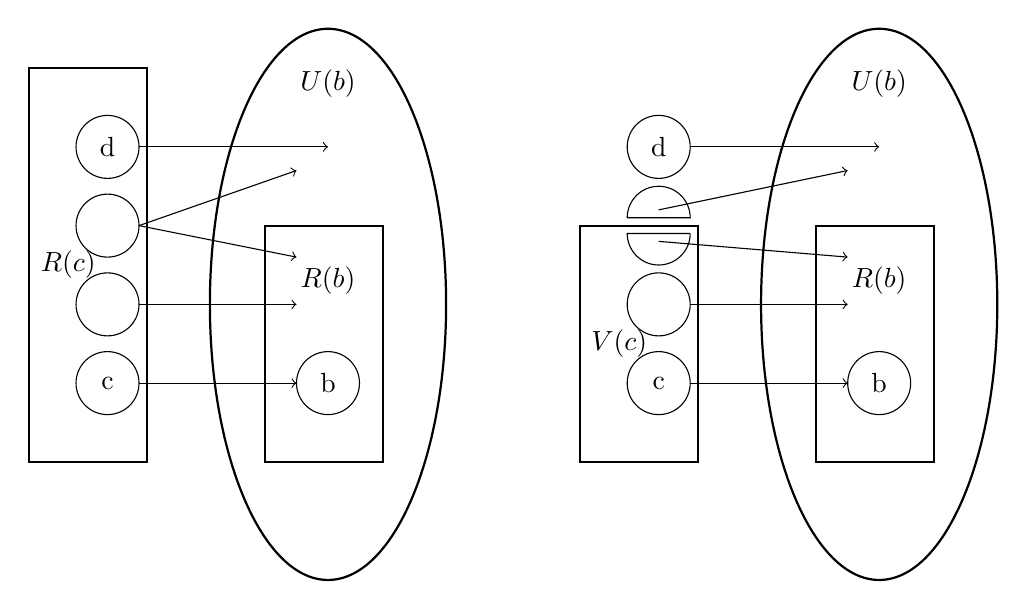
\begin{tikzpicture}
\draw (-0.5,1.5) node {$\mathscr{R}(c)$};
\draw[thick] (-1,4) rectangle (0.5,-1);
\draw (2.8,1.3) node {$\mathscr{R}(b)$};
\draw[thick] (2,2) rectangle (3.5,-1);
\draw (2.8,3.8) node {$\mathscr{U}(b)$};
\draw[thick] (2.8,1) ellipse (1.5 and 3.5);
\draw (0,0) node {c};
\draw[](0,0) circle (0.4);
\draw[](0,1) circle (0.4);
\draw[](0,2) circle (0.4);
\draw (0,3) node {d};
\draw[](0,3) circle (0.4);
\draw (2.8,0) node {b};
\draw[](2.8,0) circle (0.4);
\draw[->] (0.4,0) -- (2.4,0);
\draw[-> ] (0.4,2) -- (2.4,2.7);
\draw[-> ] (0.4,2) -- (2.4,1.6);
\draw[-> ] (0.4,1) -- (2.4,1);
\draw[-> ] (0.4,3) -- (2.8,3);

\draw (6.5,0.5) node {$\mathscr{V}(c)$};
\draw[thick] (6,2) rectangle (7.5,-1);
\draw (9.8,1.3) node {$\mathscr{R}(b)$};
\draw[thick] (9,2) rectangle (10.5,-1);
\draw (9.8,3.8) node {$\mathscr{U}(b)$};
\draw[thick] (9.8,1) ellipse (1.5 and 3.5);
\draw (7,0) node {c};
\draw[](7,0) circle (0.4);
\draw[](7,1) circle (0.4);
\draw (7,3) node {d};
\draw (7.0,2.1) -- (7.4,2.1) arc(0:180:0.4) --cycle;
\draw (7.4,1.9) -- (6.6,1.9) arc(180:360:0.4) --cycle;
\draw[](7,3) circle (0.4);
\draw (9.8,0) node {b};
\draw[](9.8,0) circle (0.4);
\draw[->] (7.4,0) -- (9.4,0);
\draw[-> ] (7,2.2) -- (9.4,2.7);
\draw[-> ] (7,1.8) -- (9.4,1.6);
\draw[-> ] (7.4,1) -- (9.4,1);
\draw[-> ] (7.4,3) -- (9.8,3);

\end{tikzpicture}
\caption{$\mathscr{R}$ is $\mathscr{U}$-stable and $\mathscr{V}$, obtained after
a split of blocks of $\mathscr{R}$ and refinement of $\mathscr{R}$, is $\mathscr{R}$-stable}
\label{fig:example-computing-simulation}
\end{figure}
Consider Figure~\ref{fig:example-computing-simulation} (taken from~\cite{cece2017foundation})
and the transition $c \rightarrow b$.
The quasiorder $\mathscr{R}$ is assumed to be $\mathscr{U}$-stable and we want
to find the coarsest simulation included in $\mathscr{R}$.
Observe that since $\mathscr{R}$ is a quasiorder the set $\mathscr{R}(c)$
is a union of blocks of $\mathscr{R}$.
A state $d$ in $\mathscr{R}(c)$ which doesn't have an outgoing transition to $\mathscr{R}(b)$
belongs to $\delta^R \circ \mathscr{U}(b)$, but cannot simulate $c$.
In order to compute the coarsest simulation included in $\mathscr{R}$ we can
remove $d$ from $\mathscr{R}(c)$.
To be efficient we want to manage \emph{blocks} of states, rather than
individual ones.
Then, the first step is a \emph{split step}, in which we split the blocks
of $\mathscr{R}$ in two groups: the ones that are are completely included
in $\delta^R \circ \mathscr{R}(b)$ and hence have a chance to simulate $c$, and
ones that are completely outside $\delta^R \circ \mathscr{R}(b)$ that then
cannot simulate $c$.
Let $\mathscr{P}$ be the equivalence relation associated to the resulting partition.
Since $\mathscr{P}$ is an equivalence, for each block of the partition that has one outgoing
transition to $\delta^R \circ (\mathscr{U} \setminus \mathscr{R})(b)$ it is
sufficient to test \emph{only for one element} of the block if it is
included in $\delta^R \circ \mathscr{R}(b)$.
For each block $E$ we call this element the \emph{representative} of $E$ and
we denote it by $E.rep$.
To perform the test in constant time we manage a counter that at first counts
the number of transitions from $E.rep$ to $\mathscr{U}(b) = \mathscr{U}([b]_{\mathscr{P}})$.
Then, we get the following equivalences:
there is no transition from $E$ to $\mathscr{R}(b)$ iff there is no transition
from $E.rep$ to $\mathscr{R}(b)$ iff this counter is null.
We can safely remove from $\mathscr{R}(c)$ those blocks of
$\delta^R \circ (\mathscr{U} \setminus \mathscr{R})(b)$ which do not have an
outgoing transition to $\mathscr{R}(b)$.
We call this step the \emph{refinement step}.
After performing it $\mathscr{R}(c)$ has been reduced to $\mathscr{V}(c)$.
Doing these split and refinement steps for all transitions from $c$ to $b$
results in the relation $\mathscr{V}$ that is a $\mathscr{R}$-stable quasiorder.

In summary, from an initial preorder we build a strictly decreasing
sequence of preorders $\{\mathscr{R}_i\}_{i \geq 0}$ such that $\mathscr{R}_{i+1}$
is $\mathscr{R}_i$-stable and contains all the simulations included in $\mathscr{R}_i$.
We observe that all the relations are finite and hence this sequence has a limit
that is reached after a finite number of steps: and we call this limit $\mathscr{R}_{sim}$.
We have that $\mathscr{R}_{sim}$ is $\mathscr{R}_{sim}$-stable.
Therefore, we observe that $\mathscr{R}_{sim}$ is a simulation and by construction
contains all simulations included in the initial quasiorder, hence is the
coarsest one and exactly corresponds to $\dir$.
We denote by $P_{\dir}$ the partition of $Q$ induced by $\dir$.
The time complexity of the algorithm proposed in~\cite{cece2017foundation}
is $O(|P_{\dir}| \cdot |\delta|)$, while it uses $O(|P_{\dir}|^2 \cdot log(|P_{\dir}|) + |Q| \cdot log(|Q|))$
space.

\textbf{Delayed and fair simulation.}
Also for the fair and the delayed simulations a wide variety of algorithms have
been proposed~\cite{clemente2017efficient,henzinger2002fair}.
Here we briefly discuss approach taken in~\cite{etessami2005fair}.
The first step is to define a \emph{parity game graph} $G_{\mathcal{B}}$ on
one \Buchi{} automaton $\mathcal{B}$ such that the winning vertices in $G_{\mathcal{B}}$
for Even (one of the two players) in the corresponding parity game determine precisely the
pairs of states $(q,q')$ of $\mathcal{B}$ where $q'$ simulates $q$.

A \emph{parity game graph} $G = \angles{V_0,V_1,E,p}$ has two disjoint sets of
vertices, $V_0$ and $V_1$ whose union is denoted by $V$.
There is an edge set $E \subseteq V \times V$, and $p: V \rightarrow \{0, \dots, d-1\}$
is a mapping that assigns a \emph{priority} to each vertex.
A \emph{parity game} on $G$, starting at vertex $v_0 \in V$, is denoted by $P(G,v_0)$,
and is played by two players, \emph{Even} and \emph{Odd}.
The play starts by placing a pebble on vertex $v_0$.
Thereafter, the pebble is moved according to the following rule: with the pebble
currently on a vertex $v_i$, and $v_i \in V_0 (V_1)$, Even (Odd, respectively)
plays and moves the pebble to a neighbour $v_{i+1}$, that is, such that
$(v_i,v_{i+1} ) \in E$.

If ever the above rule cannot be applied, i.e., someone can't move because there are
no outgoing edges, the game ends, and the player who cannot move loses.
Otherwise, the game goes on forever and defines a path
$\pi = v_0 v_1 v_2$ in $G$, called a \emph{play} of the game.
The winner of the play is determined as follows.
Let $k_{\pi}$ be the minimum priority that occurs infinitely often in the play $\pi$,
i.e., so for infinitely many $i$, $p(v_i)= k_{\pi}$ and $k_{\pi}$ is the least
number with this property.
Even wins if $k_{\pi}$ is even, whereas Odd wins if $k_{\pi}$ is odd.

We can now show how to build the parity game graph $G_{\mathcal{B}}^f$ for the
fair simulation.
We define $G_{\mathcal{B}}^f \eqdef \angles{V_0^f, V_1^f, E_{\mathcal{B}}^f, p_{\mathcal{B}}^f}$, where:
\[V_0^f  \eqdef \{ v_{(q,q',a)} \;|\; q,q' \in Q \; \wedge \;
\exists q'': q \in \delta(q'',a) \} \]
\[ V_1^f  \eqdef \{ v_{(q,q')} \;|\; q,q' \in Q \} \]
\[E_{\mathcal{B}}^f  \eqdef \{(v_{(q_1,q_1',a)}, v_{(q_1,q_2)})
\;|\; q_2' \in \delta(q_1',a)\} \; \cup \;
\{(v_{(q_1,q_1')}, v_{(q_2,q_1',a)}) \;|\; q_2 \in \delta(q_1,a)\} \]
\[p_{\mathcal{B}}^f(v) =
\begin{cases}
0 &\mbox{if } v = v_{(q,q')} \mbox{ and } q' \in F\\
1 &\mbox{if } v = v_{(q,q')} \mbox{ and } q \in F, \mbox{ and } q' \notin F\\
2 &\mbox{otherwise}\\
\end{cases}\]

We show that the defined parity game mimics the fair simulation game.
Here Odd takes the role of Spoiler, while Even takes the role of Duplicator.
When in the game the current position is node $v_{(q,q')}$, this corresponds
to the situation in which is Spoiler's turn to move, while $v_{(q,q',a)}$
denotes the situation in which is Duplicator's turn to match Spoiler's
play, that played $a$.
The priority function is defined in such a way that every
time Duplicator visits a final state, the priority function returns $0$.
It returns $1$ only if Spoiler visits a final state, but Duplicator does not.
In all other cases, $2$ is returned.
That is, Spoiler wins iff he visits an accept state infinitely often but
Duplicator does not.
It turns out that for every pair of states $q,q' \in Q$, $q \fair q'$
iff Even has a winning strategy in $P(G_{\mathcal{B}}^f, v_{(q,q')})$.

Similarly, it is possible to define the parity game graph
$G_{\mathcal{B}}^{de} \eqdef \angles{V_0^{de}, V_1^{de}, E_{\mathcal{B}}^{de}, p_{\mathcal{B}}^{de}}$
for the delayed simulation,
where:
\[V_0^{de}  \eqdef \{ v_{(b,q,q',a)} \;|\; q,q' \in Q \; \wedge \; b \in \{0,1\} \; \wedge \;
\exists q'': q \in \delta(q'',a) \} \]
\[ V_1^{de}  \eqdef \{ v_{(b,q,q')} \;|\; q,q' \in Q \; \wedge \; b \in \{0,1\}
\; \wedge \; (q' \in F \Longrightarrow b=0)\} \]
\begin{equation*}
\begin{split}
E_{\mathcal{B}}^{de} \eqdef \;
& \{(v_{(b,q_1,q_1',a)}, v_{(b,q_1,q_2')}) \;|\; q_2' \in \delta(q_1',a) \; \wedge \; q_2' \notin F \} \;\cup \\
& \{(v_{(b,q_1,q_1',a)}, v_{(0,q_1,q_2')}) \;|\; q_2' \in \delta(q_1',a) \; \wedge \; q_2' \in F \} \;\cup \\
& \{(v_{(b,q_1,q_1')}, v_{(b,q_2,q_1',a)}) \;|\; q_2 \in \delta(q_1,a) \; \wedge \; q_2 \notin F \} \;\cup \\
& \{(v_{(b,q_1,q_1')}, v_{(1,q_2,q_1',a)}) \;|\; q_2 \in \delta(q_1,a) \; \wedge \; q_2 \in F \} \\
\end{split}
\end{equation*}
\[p_{\mathcal{B}}^{de}(v) =
\begin{cases}
b &\mbox{if } v = v_{(b,q,q')}\\
2 &\mbox{if } v \in V_{\mathcal{B}}^{de}\\
\end{cases}\]

When the extra bit $b$ is equal to $1$, this corresponds to the situation in which
Spoiler encountered a final state that has not yet matched by Duplicator,
while if $b$ is equal to $0$ she matched Spoiler's final states.
The priority function assigns priority $1$ to only those vertices in $V_1$ that
signify that an unmatched final state has been visited by Spoiler.
The priority function makes sure that that the smallest number occurring infinitely
many often is $1$ iff from some point onwards the bit in the first component is $1$.
Now observe that this bit is $1$ iff a final state has been visited by Spoiler
but not yet matched by Duplicator.
In this way the winning condition of the delayed simulation game is transferred
to the parity game.
Similarly to the fair simulation parity game, it turns out that
for each pair of states $q,q' \in Q$, $q \del q'$ iff Even has a winning
strategy in $P(G_{\mathcal{B}}^{de}, v_{(q,q')})$.
We precise that in~\cite{etessami2005fair} they also define the
\emph{direct simulation parity game}.


We now describe the algorithm put forward in~\cite{jurdzinski2000small} that
solves parity games.
Later, it has been improved in~\cite{etessami2005fair}.
It uses \emph{progress measures}~\cite{klarlund1994progress,walukiewicz2000completeness}
to compute the set of vertices in a parity game from which Even has a winning strategy,
that in our case will correspond the pairs of states in the fair or delayed simulation
relation.
Let $G$ be a parity game graph with $n'$ its number of vertices and $m'$ its
number of edges.
For simulations we only need three priorities, but since the algorithm is more
general we will assume $p: V \rightarrow \{0, \dots, d-1\}$.

Let $[n] = \{0, \dots, n-1\}$ and $n_i = |p^{-1}(i)|$. We assign to each vertex a
\emph{progress measure} from $M^{\infty}_G \eqdef M_G \cup \{\infty\}$, where
\[ M_G \eqdef
\begin{cases}
[1] \times [n_1 + 1] \times [1] \times [n_3 + 1] \times \cdots \times [1] \times [n_{d-1}  1] &\mbox{if $d$ is even}\\
[1] \times [n_1 + 1] \times [1] \times [n_3 + 1] \times \cdots \times [1] \times [n_{d-2}  1] &\mbox{if $d$ is odd}\\
\end{cases} \]
That is, the progress measure is either $\infty$ or a length $d$ vector which
at even index positions is $0$, and at odd index positions $i$ ranges over $\{0, \dots, n_i\}$.
Initially, every vertex is assigned 0, the all-zero vector.
The measures are repeatedly ``incremented'' in a certain fashion until a fixed point is reached.
The \emph{increment operation} represents the heart of the algorithm.
For $i < d$ and $x \in M_G^{\infty}$ we define $\angles{x}_i$ as follows.
For $x = (l_0, \dots, l_{d-1})$, $\angles{x}_i = (l_0, \dots, l_i,0,0, \dots, 0)$.
If $x = \infty$, then $\angles{\infty}_i = \infty$.
We define a lexicographic total order on $M_G^{\infty}$, denoted $>$.
Here, index $0$ is the most significant position, and $\infty$ is greater than all other vectors.
In addition, for $d$-vectors $x$ and $y$, we write $x >_i y$ iff $\angles{x}_i > \angles{y}_i$
according to the above ordering.
Observe that $x > y$ iff $x >_{d-1} y$.
We now can define the increment operation on a progress measure:
for each $i \in [d]$, let
\[ incr_i(x) \eqdef
\begin{cases}
\angles{x}_i &\mbox{if $i$ is even, } x \neq \infty \\
min \{y \in M_G^{\infty} \;|\; y >_i x\}   &\mbox{if $i$ is odd, } x \neq \infty \\
\infty   &\mbox{if } x = \infty \\
\end{cases} \]
We observe that $incr_i$ is monotone with respect to the ordering $<$.
When $v \in V$ we abuse notation and write $\angles{x}_v$ and $incr_v(x)$ for $\angles{x}_{p(v)}$
and $incr_{p(v)}$ respectively.
For every assignment $\rho: V \rightarrow M_G^{\infty}$ of progress measures to
the vertices of a game graph, and for $v \in V$, let
\[ best\text{-}nghb\text{-}ms(\rho,v) \eqdef
\begin{cases}
\angles{min(\angles{\rho(w) \;|\; (v,w) \in E})}_v &\mbox{if } v \in V_0 \\
\angles{max(\angles{\rho(w) \;|\; (v,w) \in E})}_v &\mbox{if } v \in V_1 \\
\end{cases} \]
$best\text{-}nghb\text{-}ms$ stand for \emph{best neighbour} of $v$
with respect to the measure we defined.
We also define a \emph{lifting operator} that given an assignment $\rho$ and
$v \in V$, gives a new assignment.
First, define:
\[ update(\rho,v) \eqdef incr_v(best\text{-}nghb\text{-}ms(\rho,v)) \]
The lifted assignment, $lift(\rho,v): V \rightarrow D$, is then defined as follows:
\[ lift(\rho,v)(u) \eqdef
\begin{cases}
update(\rho,v) &\mbox{if } u=v\\
\rho(u) &\mbox{otherwise}\\
\end{cases} \]
Then, we can finally present the algorithm described in~\cite{jurdzinski2000small}.
First, for each $v \in V$ we assign to $\rho(v)$ the value 0.
Then, while there exists a $v$ such that $update(\rho,v) \neq \rho(v)$, assign
to $\rho$ the value $lift(\rho,v)$.
Let $G$ be a parity game.
In~\cite{jurdzinski2000small} they prove that Even has a winning strategy
from precisely the vertices $v$ such that, after running the lifting algorithm,
$\rho(v) < \infty$.

In~\cite{etessami2005fair} they present a more efficient version of the lifting
algorithm that maintains a set $L$ of pending vertices $v$ whose measure needs to
be considered for lifting, because a successor has recently
been updated resulting in a requirement to update $\rho(v)$.
The also maintain arrays $B$ and $C$ that store, for each vertex $v$, the value
$best\text{-}nghb\text{-}ms(\rho,v)$ and the number of successors $u$ of $v$
with $\angles{\rho(u)}_v = best\text{-}nghb\text{-}ms(\rho,v)$.
They show that the efficient implementation runs in $O(m' |M_G^{\infty}| d)$ time
and uses $O(d'm)$ space.
Going back to the original problem, that is computing the fair and the delayed
simulation, in~\cite{etessami2005fair} they show that it is possible to compute
the quasiorders in $O(|\delta||Q|^3)$ time and $O(|\delta||Q|)$ space.

As a final note, we point out that there are many tools to compute various
simulations, for example RABIT~\cite{mayrrabit} is a platform that can check the
language inclusion between two \Buchi{} automata that heavily relies on
simulation relations~\cite{abdulla2011advanced}.
Oink~\cite{Oink} is a modern tool that allows to solve parity games.
In particular, it aims to provide high-performance implementations of
state-of-the-art algorithms representing different approaches to solving parity games.
Since we showed that simulations can be characterized as parity games, Oink can
be used to efficiently compute them.



\section{Solving the language inclusion problem with complete abstractions}
\label{sec:solving-inclusion}

In this section we first give an informal introduction of the main ideas
on how to solve the language inclusion using \emph{complete abstractions}
for regular languages;
in Section~\ref{sec:checking-omega-lang-inc} we describe a framework
for solving the language inclusion problem for $\omega$-regular languages
and finally in Section~\ref{sec:checking-grammars} we describe a framework
for solving the language inclusion problem between context-free and regular
languages.

We now give a glimpse of the leading ideas that exploit abstract interpretation
techniques to design algorithms to solve the inclusion between two regular languages.
For a formal description refer to~\cite{ganty2019language}.
We remark that the reader will find the same concepts readapted in the following
sections.

Let $L_1,L_2$ be two \emph{regular} languages: we want to determine whether
$L_1 \subseteq L_2$ holds or not.
In order to do this we rely on one \emph{upper closure operator} $\rho$ (see Section~\ref{sec:order-theory}).
Intuitively, we use $\rho$ to \emph{abstract} the language $L_1$.
In fact, $\rho(L_1)$ is an \emph{over approximation} of $L_1$.
Assume that $\rho(L_2) = L_2$: we observe that in this case
$L_1 \subseteq L_2 \Longleftrightarrow \rho(L_1) \subseteq L_2$.

\begin{figure}[h]
\centering
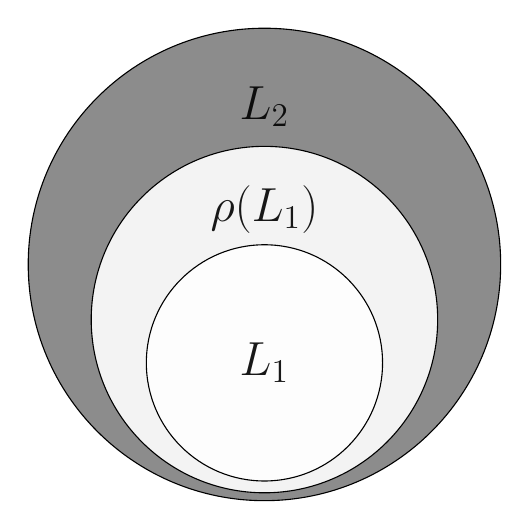
\begin{tikzpicture}
	\begin{scope} [fill opacity = .9]
    \draw[fill=gray, draw = black] (0,0) circle (3);
    \draw[fill=white, draw = black] (0,-0.7) circle (2.2);
    \draw[fill=white, draw = black] (0,-1.25) circle (1.5);
    \node at (0,2) {\LARGE\textbf{$L_2$}};
    \node at (0,0.7) {\LARGE\textbf{$\rho(L_1)$}};
    \node at (0,-1.25) {\LARGE\textbf{$L_1$}};
    \end{scope}
\end{tikzpicture}
\caption{Solving the language inclusion using one abstraction $\rho$}
\end{figure}

Let $\automa{A}$ be one FA such that $\lang{A} = L_1$.
It is well-known (and we will return on one similar concept in Section~\ref{sec:checking-omega-lang-inc}) that the language recognized
by $\mathcal{A}$ can be characterized as follows:
$\lang{A}$ equals the union of the component languages of the vector $\textrm{lfp}  (\lambda \vec{X} .
        \vec{\epsilon^F} \cup Pre_{\mathcal{A}}(\vec{X}))$ indexed by the initial states in $I$, where
$Pre_{\mathcal{A}}: \powerset(\Sigma^*)^{|Q|} \rightarrow \powerset (\Sigma^*)^{|Q|}$
is defined by $Pre_{\mathcal{A}}(\vec{X}) \overset{\triangle}{=}
\langle \bigcup_{a \in \Sigma, q \trans{a} q'} a X_{q'} \rangle_{q \in Q}$,
$\vec{\epsilon^F} \overset{\triangle}{=}
\langle \{ \epsilon \;|\; q \in F\}\rangle_{q \in Q} \in \powerset(\Sigma^*)^{|Q|}$.
In Section~\ref{sec:checking-omega-lang-inc} we give an alternative characterization
of the language recognized by an automaton which is based on a symmetric function
called $Post_{\mathcal{A}}$.
If $\rho$ is \emph{complete} for $Pre_{\mathcal{A}}$
(i.e. $\rho \circ Pre_{\mathcal{A}} \circ \rho = \rho \circ Pre_{\mathcal{A}}$),
we can characterize $\rho(L_1)$ as the union of the component languages of the vector
$\textrm{lfp}  (\lambda \vec{X} . \rho(\vec{\epsilon^F} \cup Pre_{\mathcal{A}}(\vec{X})))$
indexed by initial states in $I$.
Intuitively, \emph{completeness} models an ideal situation where no loss of precision is
accumulated in the computations of $\rho \circ Pre_{\mathcal{A}}$ when its
concrete input objects are approximated by $\rho$.
Then, the requirements for $\rho$ are:
\begin{enumerate}
\item $\rho(L_2) = L_2$;
\item $\rho$ \emph{complete} for $Pre_{\mathcal{A}}$.
\end{enumerate}

We remark that given a qoset $\angles{D, \leq}$, we defined the upper closure operator
on $D$ induced by $\leq$ as
$\rho_{\leq}(X) \overset{\triangle}{=} \{ y \in D \;|\; \exists x \in X, x \leq y\}$.
Let $\leq$ be a quasiorder on $\Sigma^*$.
It turns out that if $\leq$ is a left $L_2$-consistent qo, then $\rho_{\leq}$ meets
the previously stated requirements.
Then, if this holds, we have:
\[ L_1 \subseteq L_2 \Longleftrightarrow \rho_{\leq}(L_1) \subseteq L_2 \]
We denote by $min_{\leq}(X)$ the minor set induced by $\leq$.
The key observation is that since minor sets are finite,
$min_{\leq}(L_1)$ provides a compact representation of $\rho_{\leq}(L_1)$:
it holds that $\rho_{\leq}(L_1) \subseteq L_2 \Longleftrightarrow \forall w \in min_{\leq}(L_1), w \in L_2$,
so that:
\[ L_1 \subseteq L_2 \Longleftrightarrow \forall w \in min_{\leq}(L_1), w \in L_2 \]

\begin{figure}[h]
\centering
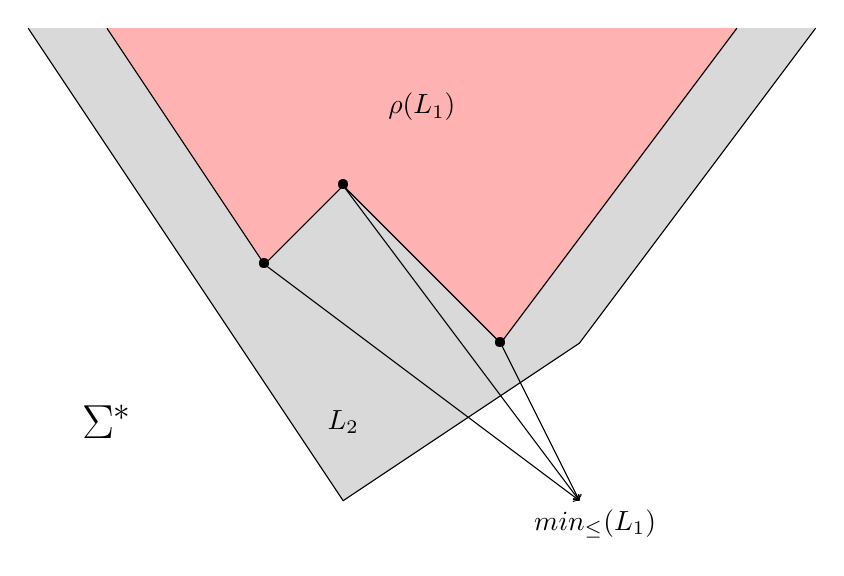
\begin{tikzpicture}
\fill[gray!30!white, draw=black] (0,6) -- (4,0) -- (7,2) -- (10,6);
\fill[red!30!white, draw=black] (1,6) -- (3,3) -- (4,4) -- (6,2) -- (9,6);
\draw (3,3) node {\textbullet};
\draw (1,1) node {\LARGE$\Sigma^*$};
\draw (4,4) node {\textbullet};
\draw (6,2) node {\textbullet};
\node at (4,1) {\textbf{$L_2$}};
\node at (5,5) {\textbf{$\rho(L_1)$}};
\draw[-> ] (3,3) -- (7,0);
\draw[-> ] (4,4) -- (7,0);
\draw[-> ] (6,2) -- (7,0);
\node at (7.2,-0.3) {$min_{\leq}(L_1)$};
\end{tikzpicture}
\caption{Representation of $L_2,\rho(L_1)$ and $min_{\leq}(L_1)$ in the qoset $\angles{\Sigma^*, \leq}$}
\label{img:aa}
\end{figure}

The final remark is that it is possible to compute $min_{\leq}(L_1)$ by
using the \texttt{Kleene} procedure to compute
$\textrm{lfp}  (\lambda \vec{X} . min_{\leq}(\vec{\epsilon^F} \cup Pre_{\mathcal{A}}(\vec{X})))$.
Exploiting \emph{complete abstractions} we have shown how to
solve the language inclusion problem: no \emph{false alarms} will be raised.

This informally summarizes the main ideas behind solving the language inclusion
for regular languages using complete abstractions.
These concepts have been generalized and adapted to solve similar problems,
namely checking the inclusion between $\omega$-regular languages and
whether the language of a CFG is contained in the one generated by a FA.
In what follows, we describe more formally how these inclusions are decided.

\subsection{Checking the inclusion between $\omega$-regular languages}
\label{sec:checking-omega-lang-inc}

Let $\mathcal{B}_1, \mathcal{B}_2$ be two B{\"u}chi automata.
To solve the \emph{language inclusion problem},
namely whether $\mathcal{L}(\mathcal{B}_1) \subseteq \mathcal{L}(\mathcal{B}_2)$ holds or not,
numerous algorithms have been proposed~\cite{abdulla2011advanced,clemente2017efficient}.
In this section we're going to describe the framework
put forward by~\cite{ganty2020omegalang}, which relies on
\emph{abstract interpretation} techniques.

One word $w \in \Sigma^{\omega}$ is \emph{ultimately periodic} iff $w = uv ^{\omega}$
for some $u \in \Sigma^*, v \in \Sigma^+$.
For $L \subseteq \Sigma^{\omega}$, $UP(L)$ denotes its subset of ultimately periodic words.
Let $L_1,L_2$ be two $\omega$-regular languages~\cite{calbrix1993ultimately}:
\[L_1 \subseteq L_2 \Longleftrightarrow UP(L_1) \subseteq UP(L_2) \]
We can represent $UP(L)$ by
$I_L \overset{\triangle}{=} \{ (u,v) \in \Sigma^* \times \Sigma^+\;
| \; uv^{\omega} \in L\}$, so that:
\[UP(L_1) \subseteq UP(L_2) \Longleftrightarrow I_{L_1} \subseteq I_{L_2}\]
Now we abstract $I_{L_1}$ using a wqo $\preceq$ on $\Sigma^* \times \Sigma^+$
such that $\rho_{\preceq}(I_{L_2}) = I_{L_2}$.

\[ I_{L_1} \subseteq I_{L_2} \Longleftrightarrow \rho_{\preceq}(I_{L_1}) \subseteq I_{L_2}\]
We define $(u,v) \equiv_{UP} (u',v')$ iff $uv^{\omega} = u' v'^{\omega}$,
where $(u,v), (u',v') \in \Sigma^* \times \Sigma^+$.
Since $\equiv_{UP}$ is a qo on $\Sigma^* \times \Sigma^+$, the closure operator
$\rho_{\equiv_{UP}}$ is well-defined.
Let $S \subseteq \Sigma^* \times \Sigma^+$ such that $\rho_{\equiv_{UP}}(S) = I_{L_1}$.
Then, $I_{L_1} \subseteq I_{L_2} \Longleftrightarrow S \subseteq I_{L_2}$
\cite{ganty2020omegalang}.
Since $\rho_{\preceq}(I_{L_2}) = I_{L_2}$ and by \emph{monotonicity} of
$\rho_{\preceq}$ we obtain:

\[ I_{L_1} \subseteq I_{L_2} \Longleftrightarrow \rho_{\preceq}(S) \subseteq I_{L_2} \]
We have to choose a suitable set $S$.
In order to do this, we rely on the automaton representation of the language $L_1$.
Let $\mathcal{B} = \langle Q, \Sigma, \delta, \{i\}, F \rangle$ be a BA with
$\mathcal{L}(\mathcal{B}) = L_1$.
Observe that in~\cite{ganty2020omegalang} they consider automata with only one
initial state.
We remark that it is always possible to construct from a BA $\automa{B}$ a
BA $\mathcal{B}' = \angles{Q \cup \{i\}, \Sigma, \delta \cup \delta', \{i\}, F}$
that has one single initial state and
accepts the same language of $\mathcal{B}$:
it is enough to add one new state $i \notin Q$,
to pick it as the only initial state and to add to $\delta$ the new
set of transitions $\delta' = \{(i,q) \;|\; \exists p \in I, q \in Q, a \in \Sigma:
q \in \delta(p,a)\}$.
For each $p,q \in Q$ we define the FA
$\mathfrak{A}_q^p \overset{\triangle}{=} \langle Q, \Sigma, \delta, \{p\}, \{q\}\rangle$,
and define $S_{\mathcal{B}} \overset{\triangle}{=} \bigcup_{p \in F}
\mathcal{L}(\mathfrak{A}^i_p) \times (\mathcal{L}(\mathfrak{A}^p_p)\setminus\{\epsilon\})$.
Since $\rho_{\equiv_{UP}} (S_{\mathcal{B}}) = I_{\lang{B}}$~\cite{ganty2020omegalang},
by the previous result:

\[ I_{\lang{B}} \subseteq I_{L_2} \Longleftrightarrow \rho_{\preceq}(S_{\mathcal{B}}) \subseteq I_{L_2} \]

We now give a \emph{least fixpoint characterization} of $S_{\mathcal{B}}$.
For all $p \in F$, the languages of the FAs $\mathfrak{A}^i_p$ and $\mathfrak{A}^p_p$
can be characterized by
$\mathcal{L}(\mathfrak{A}^i_p) = \langle \textrm{lfp} \; \lambda \vec{X} .
\vec{\epsilon^i} \cup Post_{\mathcal{B}}(\vec{X}) \rangle_{p}$ and
$\mathcal{L}(\mathfrak{A}^p_p) \setminus \{\epsilon\} = \langle \textrm{lfp} \;
\lambda \vec{X} .  \vec{\zeta^p} \cup Post_{\mathcal{B}}(\vec{X}) \rangle_{p}$
~\cite{ganty2019language}, where
$Post_{\mathcal{B}}: \powerset(\Sigma^*)^{|Q|} \rightarrow \powerset (\Sigma^*)^{|Q|}$
is defined by $Post_{\mathcal{B}}(\vec{X}) \overset{\triangle}{=}
\langle \bigcup_{a \in \Sigma, q' \trans{a} q} X_{q'}a \rangle_{q \in Q}$,
$\vec{\epsilon^i} \overset{\triangle}{=}
\langle \{ \epsilon \;|\; q = i\}\rangle_{q \in Q} \in \powerset(\Sigma^*)^{|Q|}$,
and $\vec{\zeta^p} \overset{\triangle}{=}
\langle \{ a \in \Sigma \;|\; q \in \delta (p,a)\}\rangle_{q \in Q}
\in \powerset(\Sigma^*)^{|Q|}$.
Letting $D_{1,i} \overset{\triangle}{=} \lambda \vec{X} .
\vec{\epsilon^i} \cup Post_{\mathcal{B}}(\vec{X})$ and
$D_{2,p} \overset{\triangle}{=} \lambda \vec{X} .  \vec{\zeta^p}
\cup Post_{\mathcal{B}}(\vec{X})$
we obtain that:

\[ S_{\mathcal{B}} = \bigcup_{p \in F} (\textrm{lfp} \; D_{1,i})_p \times (\textrm{lfp} \; D_{2,p})_p \]
For each $p \in F$, define the vector
$\vec{I}_{L_2}^p \in \powerset(\Sigma^* \times \Sigma^+)$
as $(\vec{I}_{L_2}^p)_q \overset{\triangle}{=} \Sigma^* \times \Sigma^+$ for $q \neq p$
and $(\vec{I}_{L_2}^p)_p \overset{\triangle}{=} I_{L_2}$.
Lift $\times$ to vectors as follows: $\vec{X} \times \vec{Y}$ is the vector
$\langle X_q \times Y_q \rangle_{q \in Q}$ where
$\vec{X} \overset{\triangle}{=}  \langle X_q \rangle_{q \in Q}$ and
$\vec{Y} \overset{\triangle}{=}  \langle Y_q \rangle_{q \in Q}$.
Let $\mathord{\leq_1} \subseteq \Sigma^* \times \Sigma^*$ and
$\mathord{\leq_2} \subseteq \Sigma^+ \times \Sigma^+$ two wqos
such that $\mathord{\preceq} = \mathord{\leq_1} \times \mathord{\leq_2}$.
This equality can be lifted to vectors.
Using this we obtain:
\[ \rho_{\preceq}(S_{\mathcal{B}}) \subseteq I_{L_2}
\Longleftrightarrow \forall p \in F, \rho_{\leq_1} (\textrm{lfp} \; D_{1,i})
\times \rho_{\leq_2}(\textrm{lfp} \; D_{2,p}) \subseteq \vec{I}_{L_2}^p\]
Observe that the least fixed points have no guarantee to converge after finitely
many steps.
We solve this issue by ``pushing'' the closure operator $\rho$ inside the fixed
point expression, and this induces no loss of precision.
This is the consequence of a property of $\rho$ relative to the function of the
fixed point expression.
A closure $\rho$ is called \emph{backward complete}, or simply \emph{complete},
for a function $f: C \rightarrow C$ when $\rho \circ f = \rho \circ f \circ \rho$.
Suppose that $\rho_{\leq_1}, \rho_{\leq_2}$ are backward complete for
$D_{1,i}$ and $ D_{2,p}$ respectively.
It implies completeness of least fixed points~\cite{cousot1979systematic}:
$\rho_{\leq_1} (\textrm{lfp} \; D_{1,i}) = \textrm{lfp} \; \rho_{\leq_1} \circ D_{1,i}$ and
$\rho_{\leq_2} (\textrm{lfp} \; D_{2,p}) = \textrm{lfp} \; \rho_{\leq_2} \circ D_{2,p}$.
Furthermore, it turns out that if one qo $\leq$ on $\Sigma^*$ is right-monotonic,
then it is also backward complete for $D_{1,i}$ and $D_{2,p}$~\cite{ganty2020omegalang}.
This implies that if $\leq_1$ and $\leq_2$ are two right-monotonic wqos:
\[ \forall p \in F, \rho_{\leq_1} (\textrm{lfp} \; D_{1,i})
\times \rho_{\leq_2}(\textrm{lfp} \; D_{2,p}) \subseteq \vec{I}_{L_2}^p
\Longleftrightarrow
\forall p \in F, \textrm{lfp} \; \rho_{\leq_1} D_{1,i}
\times \; \textrm{lfp} \; \rho_{\leq_2}  D_{2,p} \subseteq \vec{I}_{L_2}^p\]
This solves the convergence problem.
For simplicity ignore that we are working on vectors by assuming
$D_{1,i}: \powerset(\Sigma^*) \rightarrow \powerset(\Sigma^*)$.
Observe that since $\leq_1$ is a wqo,
$\langle \{ \rho_{\leq_1} (S) \;|\; S \in \powerset (\Sigma^*)\}, \subseteq \rangle$
is a complete sublattice verifying the ACC and, moreover, $\rho_{\leq_1} \circ D_{1,i}$
is a monotone function, hence it is routine to check that $\rho_{\leq_1} \circ D_{1,i}$
preserves $\cup$, and finally that
$\textrm{lfp} \; \rho_{\leq_1} \circ D_{1,i} =
\bigcup_n (\rho_{\leq_1} \circ D_{1,i})^n (\emptyset)$ for some $n \in \mathbb{N}$
by the Kleene's iterative fixed point theorem.
The same results also hold when considering $\leq_2$ and $D_{2,p}$.

We define $\gamma_{\leq_1}: \fpowerset(\Sigma^*) \rightarrow \powerset(\Sigma^*)$
such that $\gamma_{\leq_1}(Y) \overset{\triangle}{=} \rho_{\leq_1}(Y)$,
which maps finite sets of words onto upward-closed set.
Backward completeness shows that
$\rho_{\leq_1} \circ D_{1,i} \circ \gamma_{\leq_1} = \gamma_{\leq_1} \circ D_{1,i}$.
By induction we find that
$(\rho_{\leq_1} \circ D_{1,i})^n (\emptyset) = \gamma_{\leq_1}(D_{1,i}^n (\emptyset))$
for all $n \in \mathbb{N}$, hence that
$\textrm{lfp}\; \rho_{\leq_1} D_{1,i} = \gamma_{\leq_1}(D_{1,i}^N(\emptyset))$
for some $N \in \mathbb{N}$ from the convergence result on upward-closed sets
previously stated.
Observe that $D_{1,i}$ returns a finite set of words when given one,
that is, $D_{1,i}: \fpowerset(\Sigma^*) \rightarrow \fpowerset(\Sigma^*)$.
By induction we thus find that $D_{1,i}^n(\emptyset)$ is finite and effectively
computable for all $n \geq 0$.
The above reasoning also holds for $\leq_2$ and $D_{2,p}$.
Let $N_1,N_2 \in \mathbb{N}$ be such that
$(\gamma_{\leq_1}(D_{1,i}^{N_1+1}(\emptyset)))_q \subseteq
(\gamma_{\leq_1}(D_{1,i}^{N_1}(\emptyset)))_q$
and
$(\gamma_{\leq_2}(D_{2,p}^{N_2+1}(\emptyset)))_q \subseteq
(\gamma_{\leq_2}(D_{2,p}^{N_2}(\emptyset)))_q$
for all $q \in Q$.
Then, we obtain:
\[ \forall p \in F, \textrm{lfp} \; \rho_{\leq_1} D_{1,i}
\times \; \textrm{lfp} \; \rho_{\leq_2}  D_{2,p} \subseteq \vec{I}_{L_2}^p
\Longleftrightarrow
\forall p \in F, \gamma_{\leq_1}(D_{1,i}^{N_1}(\emptyset)) \times
\gamma_{\leq_2}(D_{2,p}^{N_2}(\emptyset)) \subseteq \vec{I}_{L_2}^p \]
We still have to show how to effectively detect when the sequence
$\{D_{1,i}^n(\emptyset)\}_{n \in \mathbb{N}}$ has converged, that is when
$(\gamma_{\leq_1}(D_{1,i}^{n+1}(\emptyset)))_q \subseteq
(\gamma_{\leq_1}(D_{1,i}^{n}(\emptyset)))_q$ for all $q \in Q$.
To this end define the qos $\leq_1^{\forall \exists}$ on $\fpowerset(\Sigma^*)$
such that $X \leq_1^{\forall \exists} Y \overset{\triangle}{\Longleftrightarrow}
\gamma_{\leq_1}(X) \subseteq \gamma_{\leq_1}(Y)$.
Assuming that the ordering $\leq_1$ is decidable, we find that given
$X,Y \in \fpowerset(\Sigma^*)$ we can decide $X \leq_1^{\forall \exists} Y$
by finding for each element $x \in X$ an element $y \in Y$ such that $y \leq_1 x$.
The above reasoning also holds for $\leq_2$ and $D_{2,p}$.
Finally, the lifting to vectors is an easy exercise.
Let $N_1,N_2 \in \mathbb{N}$ be such that
$(D_{1,i}^{N_1+1}(\emptyset))_q \leq_1^{\forall \exists} (D_{1,i}^{N_1}(\emptyset))_q$
and
$(D_{2,p}^{N_2+1}(\emptyset))_q \leq_2^{\forall \exists} (D_{2,p}^{N_2}(\emptyset))_q$
for all $q \in Q$ and $p \in F$.
Given $p \in F$, let $\vec{T}_p \overset{\triangle}{=} D_{1,i}^{N_1}(\emptyset)
\times D_{2,p}^{N_2}(\emptyset)$.
Observe that $\vec{T}_p$ is an effectively computable element
$(\fpowerset(\Sigma^*) \times \fpowerset(\Sigma^*))^{|Q|}$.
We have:
\[\forall p \in F, \gamma_{\leq_1}(D_{1,i}^{N_1}(\emptyset)) \times
\gamma_{\leq_2}(D_{2,p}^{N_2}(\emptyset)) \subseteq \vec{I}_{L_2}^p \Longleftrightarrow
\forall p \in F, \rho_{\preceq}(\vec{T}_p) \subseteq \vec{I}_{L_2}^p \]
Finally, since $\rho_{\preceq}$ is increasing
and $\rho_{\preceq}(I_{L_2}) = I_{L_2}$:
\[ \forall p \in F, \rho_{\preceq}(\vec{T}_p) \subseteq \vec{I}_{L_2}^p
\Longleftrightarrow
\forall p \in F, \vec{T}_p \subseteq \vec{I}_{L_2}^p\]
Observing that each element of the vector $\vec{T}_p$ is finite,
we can reduce inclusion to one finite number of membership queries:
\[\forall p \in F, \vec{T}_p \subseteq \vec{I}_{L_2}^p \Longleftrightarrow
\forall p \in F, \forall (u,v) \in (\vec{T}_p)_p, uv^{\omega} \in L_2\]
Summing up everything, we have:
\[ \lang{B} \subseteq L_2 \Longleftrightarrow
\forall p \in F, \forall (u,v) \in (\vec{T}_p)_p, uv^{\omega} \in L_2\]
Algorithms~\refPrefixes{} and~\refPeriods{} compute respectively
$D_{1,i}^{N_1}(\emptyset)$ and $D_{2,p}^{N_2}(\emptyset)$
where $N_1,N_2 \in \mathbb{N}$ are the least values such that
$(D_{1,i}^{N_1+1}(\emptyset))_q \leq_1^{\forall \exists} (D_{1,i}^{N_1}(\emptyset))_q$
and
$(D_{2,p}^{N_2+1}(\emptyset))_q \leq_2^{\forall \exists} (D_{2,p}^{N_2}(\emptyset))_q$
for all $q \in Q$ and $p \in F$.

\begin{algorithm}[h]
\phantomsection
\label{alg:prefixes}
\SetAlgorithmName{BAPrefixes}{} %last arg is the title of listing table

\SetAlgoLined
\LinesNumbered
\KwData{B{\"u}chi automaton $\mathcal{B} = \langle Q, \Sigma, \delta, \{i\}, F\rangle$}
\KwData{Procedure deciding $u \leq_1 v$, given $u,v \in \Sigma^*$}
\KwResult{$D_{1,i}^{N_1}(\emptyset)$, where
$N_1 \in \mathbb{N}$ is the least value such that $(D_{1,i}^{N_1+1}(\emptyset))_q \leq_1^{\forall \exists} (D_{1,i}^{N_1}(\emptyset))_q$
for all $q \in Q$}
$Prev \leftarrow \langle \emptyset \rangle_{q \in Q}$ \;
$done \leftarrow false$ \;
\While{$done = false$}{
    $done \leftarrow true$ \;
    $Next \leftarrow D_{1,i}(Prev)$ \;
    \ForAll{$q \in Q$}{
        \ForAll{$u \in (Next)_q$}{
            \If{$\nexists v \in (Prec)_q$ such that $v \leq_1 u$}{
                $done \leftarrow false$\;
            }
        }
    }
    \If{$done = false$}{
        $Prev \leftarrow Next$\;
    }
}
\Return $Prev$
\caption{Algorithm that computes $D_{1,i}^{N_1}(\emptyset)$, where
$N_1 \in \mathbb{N}$ is the least value such that
$(D_{1,i}^{N_1+1}(\emptyset))_q \leq_1^{\forall \exists} (D_{1,i}^{N_1}(\emptyset))_q$
for all $q \in Q$}
\end{algorithm}

\begin{algorithm}[h]
\phantomsection
\label{alg:periods}
\SetAlgorithmName{BAPeriods}{} %last arg is the title of listing table

\SetAlgoLined
\LinesNumbered
\KwData{B{\"u}chi automaton $\mathcal{B} = \langle Q, \Sigma, \delta, \{i\}, F\rangle$}
\KwData{Procedure deciding $u \leq_2 v$, given $u,v \in \Sigma^+$}
\KwData{Final state $p \in F$}
\KwResult{$D_{2,p}^{N_2}(\emptyset)$, where
$N_2 \in \mathbb{N}$ is the least value such that $(D_{2,p}^{N_2+1}(\emptyset))_q \leq_2^{\forall \exists} (D_{2,p}^{N_2}(\emptyset))_q$
for all $q \in Q$}
$Prev \leftarrow \langle \emptyset \rangle_{q \in Q}$ \;
$done \leftarrow false$ \;
\While{$done = false$}{
    $done \leftarrow true$ \;
    $Next \leftarrow D_{2,p}(Prev)$ \;
    \ForAll{$q \in Q$}{
        \ForAll{$u \in (Next)_q$}{
            \If{$\nexists v \in (Prec)_q$ such that $v \leq_2 u$}{
                $done \leftarrow false$\;
            }
        }
    }
    \If{$done = false$}{
        $Prev \leftarrow Next$\;
    }
}
\Return $Prev$
\caption{Algorithm that computes $D_{2,p}^{N_2}(\emptyset)$, where
$N_2 \in \mathbb{N}$ is the least value such that $(D_{2,p}^{N_2+1}(\emptyset))_q \leq_2^{\forall \exists} (D_{2,p}^{N_2}(\emptyset))_q$
for all $q \in Q$}
\end{algorithm}

We slightly abuse the notation calling \refPrefixes{}:
by \texttt{\refPrefixes{}($\mathcal{B}$,$\leq_1$)} we mean to invoke the procedure
\refPrefixes{} with actual parameters the automaton $\mathcal{B}$ and
\emph{the procedure} to compute $\leq_1$, and not $\leq_1$ itself because
it is an infinite relation.
The same holds for \refPeriods{} and $\leq_2$.
Finally, Algorithm~\refOmegaInc{} computes whether
$\lang{B} \subseteq L_2$ holds or not.
\begin{algorithm}[h]
\phantomsection
\label{alg:omega-lang-inc}
\SetAlgorithmName{BAInc}{} %last arg is the title of listing table
% \SetKwFunction{proc}{proc}
\SetKwProg{}{}{}{}\SetKwFunction{BAPrefixes}{BAPrefixes} \SetKwFunction{BAPeriods}{BAPeriods}

\SetAlgoLined
\LinesNumbered
\KwData{B{\"u}chi automaton $\mathcal{B} = \langle Q, \Sigma, \delta, \{i\}, F\rangle$}
\KwData{Procedure deciding $uv^{\omega} \in L_2$ given $u \in \Sigma^*, v \in \Sigma^+$}
\KwData{Decidable right-monotonic wqos $\leq_1,\leq_2$ s.t.
$\rho_{\leq_1 \times \leq_2}(I_{L_2}) = I_{L_2}$}
\KwResult{Whether $\lang{B} \subseteq L_2$ holds}
$Prefixes \leftarrow $ \BAPrefixes{$\mathcal{B}$,$\leq_1$}\;
\ForAll{$p \in F$}{
    $Periods \leftarrow $ \BAPeriods{$\mathcal{B}$, $\leq_2$, $p$} \;
    \ForAll{$u \in (Prefixes)_p$, $v \in (Periods)_p$}{
        \If{$uv^{\omega} \notin L_2$}{
            \Return \emph{false}
        }
    }
}
\Return \emph{true}
\caption{Algorithm that computes whether $\lang{B} \subseteq L_2$ holds}
\end{algorithm}


\emph{Discussion.}
We presented a framework for solving the language inclusion problem for
$\omega$-regular languages which relies on the underlying automaton representation
of the language.
% It is parametrized with two wqos $\leq_1$ and $\leq_2$ on $\Sigma^*$.
Let $\leq_1$ and $\leq_2$ be two quasiorders on $\Sigma^*$.
If the following conditions hold:
\begin{enumerate}
\item $\leq_1$ and $\leq_2$ are computable well-quasiorders;
\item $\leq_1$ and $\leq_2$ are right-monotonic;
\item $\rho_{\leq_1 \times \leq_2}(I_{L_2}) = I_{L_2}$.
\end{enumerate}
Then, $\leq_1$ and $\leq_2$ can be used in Algorithm~\refOmegaInc{}
to solve the language inclusion problem.
Observe that condition $(3)$ can be characterized alternatively as follows:

\begin{proposition}
\label{prop:rho-iff-stomega-in-lang}
$\rho_{\leq_1 \times \leq_2}(I_{L_2}) = I_{L_2}$ iff
$\forall u,s \in \Sigma^*, v,t \in \Sigma^+$
such that $uv ^{\omega} \in L_2$, $u \leq_1 s$ and $v \leq_2 t$,
it holds that $st ^{\omega} \in L_2$.
\end{proposition}

\begin{proof}
If $\rho_{\leq_1 \times \leq_2}(I_{L_2}) = I_{L_2}$, then
consider $u,s \in \Sigma^*, v,t \in \Sigma^+$ such that
$uv \in L_2$, $u \leq_1 s$ and $v \leq_2 t$.
By definition of $\rho$, $s \in \rho_{\leq_1}(u)$ and $t \in \rho_{\leq_2}(v)$,
so that $(s,t) \in \rho_{\leq_1 \times \leq_2}(I_{L_2})$ and by hypothesis
$\rho_{\leq_1 \times \leq_2}(I_{L_2}) = I_{L_2}$.
Since $I_{L_2} = \{ (w_1,w_2) \;|\; w_1w_2^{\omega} \in L_2\}$,
$st ^{\omega} \in L_2$.

For the other implication we proceed by showing:
(i) $\rho_{\leq_1 \times \leq_2}(I_{L_2}) \subseteq I_{L_2}$;
(ii) $ I_{L_2} \subseteq \rho_{\leq_1 \times \leq_2}(I_{L_2})$.
Let $(s,t) \in \rho_{\leq_1 \times \leq_2}(I_{L_2})$, then
$\exists (u,v) \in I_{L_2}$ such that $u \leq_1 s$ and $v \leq_2 t$.
Then, by hypothesis, $st ^{\omega} \in L_2$, so that $(s,t) \in I_{L_2}$.
Let $(s,t) \in I_{L_2}$.
We observe that by reflexivity of $\leq_1$ and $\leq_2$
it holds that $\forall w_1 \in \Sigma^*, w_1 \in \rho_{\leq_1}(w_1)$ and
$\forall w_2 \in \Sigma^+, w_2 \in \rho_{\leq_2}(w_2)$.
This implies that $(s,t) \in \rho_{\leq_1 \times \leq_2}(I_{L_2})$.
\end{proof}

Observe that the performance of Algorithm~\refOmegaInc{} depends on
the choice of the two wqos $\leq_1$ and $\leq_2$.
Let $\mathord{\preceq_1} \subseteq \mathord{\leq_1}$, then
\texttt{\refPrefixes{}($\mathcal{B}$,$\leq_1$)} will converge in less iterations
than \texttt{\refPrefixes{}($\mathcal{B}$,$\preceq_1$)}, because the condition
at line $8$ will result false more often.
The same holds for \refPeriods{}.
This implies that we want to consider coarser relations in order to let the
algorithm converge faster.

\begin{definition}
\label{def:lang-cover}
Let $\leq_1, \leq_2$ a pair of qos on $\Sigma^*$.
We say that the pair $\leq_1,\leq_2$ \emph{covers} an $\omega$-regular language $L$ iff:
\[ L = \bigcup_{uv ^{\omega} \in L} \rho_{\leq_1}(u) \rho_{\leq_2}(v)^{\omega} \]
\end{definition}

In~\cite{ganty2020omegalang} they observe that if $\leq_1,\leq_2$ covers one language,
then $\rho_{\leq_1 \times \leq_2}(I_{L_2}) = I_{L_2}$.
They also propose some wqos that meet the requirements of the framework.
First, we define the \emph{state-based} wqos.
Let $u,v \in \Sigma^*$ and $\mathcal{B}$ be a BA.
\[ u \leq_{\mathcal{B}}^1 v \overset{\triangle}{\Longleftrightarrow}
ctx_{\mathcal{B}}(u) \subseteq ctx_{\mathcal{B}}(v)\]

\[ u \leq_{\mathcal{B}}^2 v \overset{\triangle}{\Longleftrightarrow}
u \leq^1_{\mathcal{B}} v \; \wedge \;
ctx_{\mathcal{B}}^F(u) \subseteq ctx_{\mathcal{B}}^F(v)\]

\[ u \leq_{\mathcal{B}}^r v \overset{\triangle}{\Longleftrightarrow}
post^{\mathcal{B}}_u(I) \subseteq post^{\mathcal{B}}_v(I)\]

Observe that $\wss{B}$ has been already defined in Section~\ref{sec:qos-on-words}.
It holds that $\leq_{\mathcal{B}}^1$ and $\leq_{\mathcal{B}}^2$ are monotonic, while
$\leq_{\mathcal{B}}^r$ is right-monotonic.
Furthermore, the pairs $\leq_{\mathcal{B}}^1, \leq_{\mathcal{B}}^2$ and
$\leq_{\mathcal{B}}^r, \leq_{\mathcal{B}}^2$ cover $\lang{B}$, so that they can
be used to instantiate the Algorithm~\refOmegaInc{}.

Next, we define the \emph{syntactic quasiorders}.
Let $L \subseteq \Sigma^{\omega}$.
For $u \in \Sigma^*$ define
$c_L \overset{\triangle}{=} \{(x,y,r) \in \Sigma^{*3} \;|\; xuyr^{\omega} \in L\}$,
$d_L \overset{\triangle}{=} \{(s,t) \in \Sigma^{*2} \;|\; s(ut) ^{\omega} \in L\}$ and
$e_L \overset{\triangle}{=} \{ (s,t) \in \Sigma^{*2} \;|\; ust ^{\omega} \in L\}$.
We define:
\[ u \leq^1_L v \overset{\triangle}{\Longleftrightarrow} c_L(u) \subseteq c_L(v) \]
\[ u \leq^2_L v \overset{\triangle}{\Longleftrightarrow} c_L(u) \subseteq c_L(v)
\; \wedge \; d_L(u) \subseteq d_L(v)\]
\[ u \leq^r_L v \overset{\triangle}{\Longleftrightarrow} e_L(u) \subseteq e_L(v) \]

It holds that $\leq_{L}^1$ and $\leq_{L}^2$ are monotonic, while
$\leq_{L}^r$ is right-monotonic.
They are computable wqos,
and the pairs $\leq_{L}^1, \leq_{L}^2$ and
$\leq_{L}^r, \leq_{L}^2$ cover $L$, so that they can
be used to instantiate the Algorithm~\refOmegaInc{}.
Let $\mathcal{B}$ be a BA such that $L = \lang{B}$.
It holds that
$\mathord{\leq^1_{\mathcal{B}}} \subseteq \mathord{\leq^1_L}$,
$\mathord{\leq^2_{\mathcal{B}}} \subseteq \mathord{\leq^2_L}$ and
$\mathord{\leq^r_{\mathcal{B}}} \subseteq \mathord{\leq^r_L}$.
Observe that furthermore in~\cite{ganty2020omegalang} they also prove the following:

\begin{proposition}
\label{proposition:synt-largest}
Let $\leq_1,\leq_2$ be a pair of qos covering $L$ such that $\mathord{\leq_2} \subseteq \mathord{\leq_1}$.
\begin{itemize}
\item If $\leq_1, \leq_2$ are both monotonic, then $\mathord{\leq_1} \subseteq \mathord{\leq^1_L}$
and $\mathord{\leq_2} \subseteq \mathord{\leq^2_L}$;
\item If $\leq_1$ is right-monotonic, and $\leq_2$ is monotonic then
$\mathord{\leq_1} \subseteq \mathord{\leq^1_L}$
and $\mathord{\leq_2} \subseteq \mathord{\leq^2_L}$.
\end{itemize}
\end{proposition}

We observe the following:
\begin{proposition}
\label{prop:forall-stronger-coverage}
Let $\mathcal{B}$ be a BA.
Let $\leq_1,\leq_2$ be a pair of qos such that
$\forall u,s \in \Sigma^*, v,t \in \Sigma^+$, if
$uv ^{\omega} \in \lang{B}$, $u \leq_1 s$ and $v \leq_2 t$,
then $st ^{\omega} \in \lang{B}$.
Then, $\leq_1,\leq_2$ \emph{covers} $\lang{B}$.
\end{proposition}

\begin{proof}
Let $L = \bigcup_{uv ^{\omega} \in \lang{B}} \rho_{\leq_1}(u) \rho_{\leq_2}(v)^{\omega}$.
We have to show that $L = \lang{B}$.
That $\lang{B} \subseteq L$ holds is implied by the fact that $\leq_1$ and $\leq_2$
are qos, so that they are reflexive.
That $L \subseteq \lang{B}$ holds is implied by the hypothesis
that $\forall uv ^{\omega} \in \lang{B}$, if $s \in \Sigma^*, t \in \Sigma^+$
are such that $u \leq_1 s$ and $v \leq_2 t$, then $st ^{\omega} \in \lang{B}$.
This implies, by definition of $L$, that each element in $L$ is also in $\lang{B}$.
\end{proof}


In Chapter~\ref{chap:qos} we propose some suitable
relations on words that can fit the described framework.
We will show that defining quasiorders on words that are based on simulations
we obtain relations that are coarser than the state-based ones,
while being finer than the syntactic qos, effectively lying the in
the middle between the two categories of preorders.
In Chapter~\ref{chap:examples} we give some examples that show the practical
advantage of using simulation-based qos.

\begin{figure}[h]
\centering
\begin{tikzpicture}[shorten >=1pt,node distance=3cm,auto]
  \tikzstyle{every state}=[fill={rgb:black,1;white,10}]
  \node[state,initial] (q_0) {$q_0$};
  \node[state,accepting] (q_1) [right of=q_0]  {$q_1$};
  \path[->]
  (q_0) edge [loop above] node {$a,b$} (q_0)
  (q_0) edge node {$a$} (q_1)
  (q_1) edge [loop above] node {$a$} (q_1)
  ;
\end{tikzpicture}
\caption{B{\"u}chi automaton that accepts the language $(a+b)^*a^{\omega}$}
\label{fig:BA-example-2}
\end{figure}

\begin{figure}[h]
\centering
\begin{tikzpicture}[shorten >=1pt,node distance=3cm,auto]
  \tikzstyle{every state}=[fill={rgb:black,1;white,10}]
  \node[state,initial] (q_0) {$q_0$};
  \node[state,accepting] (q_1) [right of=q_0]  {$q_1$};
  \path[->]
  (q_0) edge [bend left] node {$a$} (q_1)
  (q_1) edge [bend left] node {$b$} (q_0)
  ;
\end{tikzpicture}
\caption{B{\"u}chi automaton that accepts the language $(ab)^{\omega}$}
\label{fig:BA-example-3}
\end{figure}

\begin{example}
We now give an example of a run of Algorithm~\refOmegaInc{}.
Let $\mathcal{B}$ be the BA in Figure~\ref{fig:BA-example-2} and $\mathcal{B}'$
be the BA in Figure~\ref{fig:BA-example-3}.
We want to decide whether $\lang{B} \subseteq \lang{B'}$ holds or not.
For this example, we instantiate the algorithm with the state-based qos
$\wss{B}, \wssf{B}$.

The first step is to compute the vector $Prefixes$, calling the
procedure \texttt{\refPrefixes{}($\mathcal{B}$,$\wss{B}$)}.
Table~\ref{table:ex-run-D1} shows the first three Kleene's iterates of the function
$\Di{q_0}$ relative to $\mathcal{B}$.
We point out some of the relations between words based on $\wss{B}$.
Observe that $\ctx{B}{a} = \{(q_0,q_0),(q_0,q_1),(q_1,q_1)\}$ and
$\ctx{B}{b} = \{(q_0,q_0)\}$.
Since $\ctx{B}{aa} = \{(q_0,q_0),(q_0,q_1),(q_1,q_1)\}$, we observe that
$\ctx{B}{a} \subseteq \ctx{B}{aa}$ so that $a \wss{B} aa$.
Similarly, $\ctx{B}{ab} = \ctx{B}{bb} = \{(q_0,q_0)\}$, hence
$b \wss{B} ab$ and $b \wss{B} bb$.
Finally, $\ctx{B}{ba} = \{(q_0,q_0),(q_0,q_1)\}$ and then $b \wss{B} ba$.
Consider $\Dine{q_0}{3}{q_0}$.
By the previous observations we can verify that $\forall u \in \Dine{q_0}{3}{q_0}$,
$\exists v \in \Dine{q_0}{2}{q_0}$ such that $v \wss{B} u$.
Furthermore, it also holds that $\forall u \in \Dine{q_0}{3}{q_1}$,
$\exists v \in \Dine{q_0}{2}{q_1}$ such that $v \wss{B} u$.
Hence, \texttt{\refPrefixes{}($\mathcal{B}$,$\wss{B}$)} returns the vector
$(\{a,b\}, \{a\})$.

\begin{table}[h]
\centering
\begin{tabular}{ c | c | c }
 & $q_0$ & $q_1$ \\
\hline
$D_{1,q_0}^0(\emptyset)$ & $\emptyset$ & $\emptyset$ \\
$D_{1,q_0}^1(\emptyset)$ & $\{\epsilon\}$ & $\emptyset$ \\
$D_{1,q_0}^2(\emptyset)$ & $\{\epsilon, a, b\}$ & $\{a\}$ \\
$D_{1,q_0}^3(\emptyset)$ & $\{\epsilon, a, b, aa, ab, ba, bb\}$ & $\{a, aa\}$ \\
\end{tabular}
\caption{The first three Kleene's iterates of $D_{1,q_0}$ on the automaton in Figure~\ref{fig:BA-example-2}}
\label{table:ex-run-D1}
\end{table}

The second step is to compute, for each final state, the vector $Periods$.
Since there is just one final state, we now consider the only call to
\texttt{\refPeriods{}($\mathcal{B}$, $\wssf{B}$)}.
Table~\ref{table:ex-run-D2} shows the first two Kleene's iterates of the function
$\Dp{q_1}$ relative to $\mathcal{B}$.
We observe that $\ctxf{B}{a} = \{(q_0,q_1), (q_1,q_1)\}$ and $\ctxf{B}{aa} = \{(q_0,q_1),(q_1,q_1)\}$
so that $\ctxf{B}{a} \subseteq \ctxf{B}{aa}$ and $\ctx{B}{a} \subseteq \ctx{B}{aa}$.
This implies $a \wssf{B} aa$, so that $\forall u \in \Dpne{q_1}{2}{q_1}$
$\exists v \in \Dpne{q_1}{1}{q_1}$ such that $v \wssf{B} u$.
Hence, \texttt{\refPeriods{}($\mathcal{B}$, $\wssf{B}$)} returns the vector $(\emptyset, \{a\})$.

\begin{table}[h]
\centering
\begin{tabular}{ c | c | c }
 & $q_0$ & $q_1$ \\
\hline
$D_{2,q_1}^0(\emptyset)$ & $\emptyset$ & $\emptyset$ \\
$D_{2,q_1}^1(\emptyset)$ & $\emptyset$ & $\{a\}$ \\
$D_{2,q_1}^2(\emptyset)$ & $\emptyset$ & $\{a, aa\}$ \\
\end{tabular}
\caption{The first two Kleene's iterates of $D_{2,q_1}$ on the automaton in Figure~\ref{fig:BA-example-2}}
\label{table:ex-run-D2}
\end{table}

The last step is to compute whether $\forall u \in \Dine{q_0}{2}{q_1}=\{a\}, v \in \Dpne{q_1}{1}{q_1} = \{a\}$
it holds that $uv ^{\omega} \in \lang{B'}$.
Since $a ^{\omega} \notin \lang{B'}$, the algorithm terminates and returns \texttt{false}:
$\lang{B} \nsubseteq \lang{B'}$.
\end{example}

\subsection{Checking the language inclusion between regular and context-free languages}
\label{sec:checking-grammars}

In this Section we describe the framework put forward in~\cite{ganty2019language}
to check whether one context-free language $L_1$ is contained in a regular
language $L_2$.
We remark that our main interest is in the language inclusion between $\omega$-regular
languages, but it turns out that the qo that we define in Definition~\ref{defn:wsdir}
can be plugged in this framework to solve whether the language of a context-free
grammar is included in a regular one.

Let $\mathcal{G} = \angles{\mathcal{V},\Sigma,P}$ be a CGF in CNF
where $\mathcal{V} = \{X_0, \dots, X_n\}$.
First, observe that $\mathcal{G}$ induces the following set of equations:
\[ Eqn(\mathcal{G}) \eqdef \{X_i = \cup_{X_1 \rightarrow \beta_j \in P}
\; \beta_j \;|\; i \in [0,n]\} \]
Given a subset of variables $S \subseteq \mathcal{V}$ of a grammar, the set of
words generated from some variable in $S$ is defined as
$W_S^{\mathcal{G}} \eqdef \{w \in \Sigma^* \;|\; \exists X \in S, X \rightsquigarrow w\}$.
When $S = \{X\}$ we slightly abuse the notation and write $W_X^{\mathcal{G}}$.
Observe that $\lang{G} = W_{X_0}^{\mathcal{G}}$.

In order to give a \emph{least fixpoint characterization} of the language of $\mathcal{G}$
we define the vector $\vec{b} \in \powerset (\Sigma^*)^{|\mathcal{V}|}$ and
the function $Fn_{\mathcal{G}}: \powerset (\Sigma^*)^{|\mathcal{V}|} \rightarrow  \powerset (\Sigma^*)^{|\mathcal{V}|}$:
\[  \vec{b} \eqdef \angles{b_i}_{i \in [0,n]}
\textrm{ where } b_i \eqdef \{\beta \;|\; X_i \rightarrow \beta \in P, \beta \in \Sigma \cup \{\epsilon\} \}\]
\[ Fn_{\mathcal{G}}(\angles{X_i}_{i \in [0,n]}) \eqdef \angles{\beta_1^{(i)} \cup \dots \cup \beta_n^{(i)}}_{i \in [0,n]}
\textrm{ where } \beta_j^{(i)} \in \mathcal{V}^2 \textrm{ and } X_i \rightarrow \beta_j^{(i)} \in P\]

We remark that $\lambda \vec{X}. \; \vec{b} \cup Fn_{\mathcal{G}}(\vec{X})$ is a well-defined
monotonic function in $\powerset(\Sigma^*)^{|\mathcal{V}|} \rightarrow \powerset(\Sigma^*)^{|\mathcal{V}|}$,
which therefore has the least fixpoint
$\angles{Y_i}_{i \in [0,n]} = \lfp (\lambda \vec{X}. \; \vec{b} \cup Fn_{\mathcal{G}}(\vec{X}))$.
It is well-known~\cite{ginsburg1962two} that the language $\lang{G}$
accepted by $\mathcal{G}$ is such that $\lang{G} = Y_0$.
Let $L_2$ be a language, we define $\angles{\vec{L}_2^{X_0}}_{0} \eqdef L_2$
and $\angles{\vec{L}^{X_0}_2}_{i \in [1,n]} \eqdef \Sigma^*$.
It turns out that:
\[ \lang{G} \subseteq L_2 \Longleftrightarrow \lfp(\lambda \vec{X}. \; \vec{b} \cup
Fn_{\mathcal{G}}(\vec{X})) \subseteq \vec{L}_2^{X_0} \]

Similarly to Section~\ref{sec:checking-omega-lang-inc}, backward completeness
is again linked to effectively checking the language inclusion.
Let $\rho$ be a upper closure operator on $\Sigma^*$.
In~\cite{ganty2019language} they show that if $\rho$ is backward complete for
both $\lambda X.Xa$ and $\lambda X. aX$ for all $a \in \Sigma$, then $\rho$ is
backward complete for $Fn_{\mathcal{G}}$ and $\gfunclambda$.
It turns out that if $\rho$ is backward complete for $\gfunclambda$, then:
\[ \rho( \lfp (\gfunclambda) ) = \lfp (\lambda \vec{X}. \rho(\gfunc))\]
Furthermore, if $\rho$ is backward complete for left and right concatenation
and $\rho(L_2)= L_2$, then we have that:
\[ \lang{G} \subseteq L_2 \Longleftrightarrow \lfp (\lambda \vec{X}. \rho(\gfunc)) \subseteq \vec{L}_2^{X_0} \]

We recall that a \emph{Galois Connection} (GC) between two posets
$\angles{C,\leq_C}$ (called \emph{concrete domain}) and $\angles{A, \leq_A}$
(called \emph{abstract domain}) consists of two functions
$\alpha : C \rightarrow A$ and $\gamma : A \rightarrow C$ such that
$\alpha(c) \leq_A a \Longleftrightarrow c \leq_C \gamma (a)$ holds for all
$c \in C$ and $a \in A$.
A GC is denoted by $\gc{C}{\leq_C}{A}{\leq_A}$.
If $C$ or $A$ is a qoset, $\gc{C}{\leq_C}{A}{\leq_A}$ is a
\emph{quasiorder Galois Connection} (QGC).


The following Theorem relies on the equivalence
$\lang{G} \subseteq L_2 \Longleftrightarrow \lfp (\lambda \vec{X}. \rho(\gfunc)) \subseteq \vec{L}_2^{X_0}$,
but formulated on GCs rather than closures.
In particular, it shows how to design an algorithm that solves $\lang{G} \subseteq L_2$
on an abstraction $D$ of the concrete domain $\angles{\powersetSigmas, \subseteq}$
whenever $D$ satisfies a list of requirements related to backward completeness
and computability.
\begin{theorem}
\label{theorem:compute-cfg}
Let $\mathcal{G}$ be a CFG in CNF and let $L_2$ be a language over $\Sigma$.
Let $\gc{\powerset(\Sigma^*)}{\subseteq}{D}{\leq_D}$ be a GC where $\angles{D, \leq_D}$
is a poset.
Assume that the following properties hold:
\begin{enumerate}
\item $L_2 \in \gamma(D)$ and for every $a \in \Sigma, x \in \powerset (\Sigma^*)$,
$\gamma(\alpha(aX)) = \gamma(\alpha(a\gamma(\alpha(X))))$ and
$\gamma(\alpha(Xa)) = \gamma(\alpha(\gamma(\alpha(X))a))$;
\item $\angles{D, \leq_D, \sqcup, \bot_D}$ is an \emph{effective domain}, meaning that
$\angles{D, \leq_D, \sqcup, \bot_D}$ is an ACC join-semilattice with bottom
$\bot_D$, every element of $D$ has a finite representation, the binary relation
$\leq_D$ is decidable and the binary lub $\sqcup$ is computable;
\item There is an algorithm, say $Fn^{\sharp}(\vec{X}^{\sharp})$,
which computes $\alpha(Fn_{\mathcal{G}}(\gamma(\vec{X})))$, for all
$\vec{X}^{\sharp} \in \alpha(\powerset(\Sigma^*)^{|\mathcal{V}|})$;
\item There is an algorithm, say $\vec{b}^{\sharp}$, which computes $\alpha(\vec{b})$;
\item There is an algorithm, say $Incl^{\sharp}(\vec{X}^{\sharp})$, which decides
the abstract inclusion $\vec{X}^{\sharp} \leq_D \alpha(\vec{L}_2^{X_0})$,
for all $\vec{X}^{\sharp} \in \alpha(\powerset(\Sigma^*)^{|\mathcal{V}|})$.
\end{enumerate}
Then, the following is an algorithm which decides whether $\lang{G} \subseteq L_2$:
\[
\begin{cases}
\angles{Y_i^{\sharp}}_{i \in [0,n]} \leftarrow \textrm{ \emph{\texttt{Kleene(}}}
\lambda \vec{X}^{\sharp}. (\vec{b}^{\sharp} \cup Fn^{\sharp}_{\mathcal{G}}(\vec{X})), \vec{\bot}_D \textrm{\emph{\texttt{)}} } \\
\textrm{ \emph{\textbf{return }}} Incl^{\sharp}(\angles{Y_i^{\sharp}}_{i \in [0,n]})
\end{cases}\]
\end{theorem}

Theorem~\ref{theorem:compute-cfg} is parametric on the effective
domain $D$ that can be used to instantiate it.
Let $\leq$ be a quasiorder on $\Sigma^*$.
In~\cite{ganty2019language} they observe that the qoset of
antichains $\angles{AC_{\angles{\Sigma^*,\leq}}, \sqsubseteq}$ can be viewed as an abstraction
of the concrete domain of all languages $\powerset(\Sigma^*)$ as follows.
The maps $\alpha_{\leq}: \powersetSigmas \rightarrow \acSigmas$ and
$\gamma_{\leq}: \acSigmas \rightarrow \powersetSigmas$ are defined by:
\[ \alpha_{\leq}(X) \eqdef \minor{X} \]
\[ \gamma_{\leq}(X) \eqdef \rho_{\leq}(X) \]
Where $\alpha_{\leq}(X)$ is meant to return \emph{any} minor set of the language $X$
since minors are not unique.
It turns out that $\pgc{\powersetSigmas}{\subseteq}{\acSigmas}{\sqsubseteq}{\alpha_{\leq}}{\gamma_{\leq}}$
is a QGC and $\gamma_{\leq} \circ \alpha_{\leq} = \rho_{\leq}$.
Since by definition $\alpha_{\leq}(X) = \minor{X}$, and $\minor{X}$ is
\emph{finite} (see Section~\ref{sec:order-theory}), the QGC $\pgc{\powersetSigmas}{\subseteq}{\acSigmas}{\sqsubseteq}{\alpha_{\leq}}{\gamma_{\leq}}$
allows us to represent and manipulate $\leq$-upward closed sets in $\powersetSigmas$
using finite subsets.
Furthermore, they prove that if $\leq$ is a $L_2$-consistent well-quasiorder
(see Section~\ref{sec:qos-on-words}),
Algorithm~\refGrammar{} solves whether $\lang{G} \subseteq L_2$ holds.

\begin{algorithm}[h]
\phantomsection
\label{alg:grammar}
\SetAlgorithmName{CFGInc}{}

\SetAlgoLined
\LinesNumbered
\KwData{CGF $\mathcal{G} =\angles{\mathcal{V}, \Sigma, P}$}
\KwData{Procedure deciding $u \in L_2$, given $u \in \Sigma^*$}
\KwData{Decidable $L_2$-consistent wqo $\leq$}
\KwResult{Whether $\lang{G} \subseteq L_2$ holds}

$\angles{Y_i^{\sharp}}_{i \in [0,n]} \leftarrow$ \texttt{Kleene($\lambda \vec{X}. (\minor{\vec{b}} \cup \minor{Fn_{\mathcal{G}}(\vec{X}))}$, $\angles{\emptyset}_{i \in [0,n]}$)} \;
\ForAll{$u \in Y_0$}{
    \If{$u \notin L_2$}{
        \Return false\;
    }
}
\Return true
\caption{Algorithm that computes whether $\lang{G} \subseteq L_2$ holds}
\end{algorithm}

Let $\mathcal{A}$ be a FA.
In~\cite{ganty2019language} they observe that $\leq^1_{\mathcal{A}}$ and $\leqq_{\lang{A}}$
(see Section~\ref{sec:qos-on-words}) are monotonic $\lang{A}$-consistent
computable wqos that can be used to instantiate Algorithm~\refGrammar{}
in order to solve the language inclusion problem between context-free and
regular languages.

Even if we are mainly interested in the language inclusion problem between
$\omega$-regular languages, we show that the quasiorder defined in Definition~\ref{defn:wsdir}
is a $L_2$-consistent computable wqo when $L_2$ is regular,
and then it can be used to instantiate Algorithm~\refGrammar{}.

\begin{example}
(Taken from~\cite{ganty2019language})
\sloppy Let $\sloppy\mathcal{G} = \angles{\{X_0,X_1\}, \{a,b\}, \{X_0 \rightarrow X_0X_1 | X_1X_0 | b, X_1 \rightarrow a\}}$
a CFG in CNF and $\mathcal{A}$ the automaton in Figure~\ref{fig:example-grammar}.
For this example, we instantiate the algorithm~\refGrammar{} with the
state-based quasiorder $\wss{A}$.
First, we observe some relations between words induced by $\wss{A}$.
Observe $\ctx{A}{\epsilon} = \ctx{A}{a} = \ctx{A}{b} = \ctx{A}{aa} = \{(q_0,q_0), (q_1,q_1), (q_2,q_2)\}$,
moreover $ \ctx{A}{ab} = \ctx{A}{a}$ and $\ctx{A}{ba} = \ctx{A}{aa} = \ctx{A}{baa} = \ctx{A}{aab} = \ctx{A}{aba} = \{(q_0,q_2),(q_1,q_2),(q_2,q_2)\}$.
We show the first three Kleene iterates computed by Algorithm~\refGrammar{}
using the qo $\wss{A}$:
\begin{equation*}
\begin{split}
\vec{Y}^{(0)} & = \angles{\emptyset, \emptyset} \\
\vec{Y}^{(1)} & = \minor{\vec{b}} = \angles{\{b\},\{a\}} \\
\vec{Y}^{(2)} & = \minor{\vec{b}} \sqcup \minor{Fn_{\mathcal{G}}(\vec{Y}^{(1)})} = \angles{\minor{\{ba,ab,b\}},\minor{\{a\}}} = \angles{\{ba,ab,b\},\{a\}} \\
\vec{Y}^{(3)} & = \minor{\vec{b}} \sqcup \minor{Fn_{\mathcal{G}}(\vec{Y}^{(2)})} = \angles{\minor{\{ba,ab,b\}},\minor{\{a\}}} = \angles{\{ba,ab,b\},\{a\}} \\
\end{split}
\end{equation*}
So that the least fixpoint is $\vec{Y} = \angles{\{ba,ab,b\},\{a\}}$.
Since $ab \in (\vec{Y})_0$ but $ab \notin \lang{A}$, Algorithm~\refGrammar{}
derives $\lang{G} \nsubseteq \lang{A}$.
\end{example}

\begin{figure}[h]
\centering
\begin{tikzpicture}[shorten >=1pt,node distance=3cm,auto]
  \tikzstyle{every state}=[fill={rgb:black,1;white,10}]
  \node[state,initial] (q_0) {$q_0$};
  \node[state] (q_1) [right of=q_0]  {$q_1$};
  \node[state,accepting] (q_2) [right of=q_1]  {$q_2$};
  \path[->]
  (q_0) edge node {$a$} (q_1)
  (q_1) edge node {$a$} (q_2)
  (q_1) edge [loop above] node {$b$} (q_1)
  (q_2) edge [loop above] node {$a,b$} (q_2)
  (q_0) edge [bend right] node {$b$} (q_2)
  ;
\end{tikzpicture}
\caption{Automaton that accepts the language $(b + ab^*a)(a+b)^*$}
\label{fig:example-grammar}
\end{figure}
